\documentclass[11pt, a4paper]{article} %or article has only section and below, book and report also have chapter: http://texblog.org/2007/07/09/documentclassbook-report-article-or-letter/
\usepackage{float}
\usepackage[utf8]{inputenc} % use utf8 encoding of symbols such as umlaute for maximal compatibility across platforms
\usepackage{caption} % provides commands for handling caption sizes etc.
%\usepackage[a4paper, left=25mm, right=20mm, top=25mm, bottom=20mm]{geometry} % to easily change margin widths: https://www.sharelatex.com/learn/Page_size_and_margins
\usepackage[bottom]{footmisc} % I love footnotes! And they should be down at the bottom of the page!
\usepackage{graphicx} % when using figures and alike
\usepackage[hidelinks]{hyperref} % for hyperreferences (links within the document: references, figures, tables, citations)
\usepackage{euler} % a math font, only for equations and alike; call BEFORE changing the main font; alternatives: mathptmx, fourier,
%\usepackage{gentium} % for a different font; you can also try: cantarell, charter, libertine, gentium, bera, ... http://tex.stackexchange.com/questions/59403/what-font-packages-are-installed-in-tex-live
%------------------------------------------------------------------------------------------------------
%------- text size settings --------------
\setlength{\textwidth}{16cm}%
\setlength{\textheight}{25cm} %23
%(these values were used to fill the page more fully and thus reduce the number of pages!)
\setlength{\topmargin}{-1.5cm} %0
\setlength{\footskip}{1cm} %
%\setlength{\hoffset}{0cm} %
\setlength{\oddsidemargin}{1cm}%
\setlength{\evensidemargin}{-.5cm}%
\setlength{\parskip}{0cm} % Abstand zwischen Absätzen
% ----------------------------------------------------------------
\renewcommand{\textfraction}{0.1} % allows more space to graphics in float
\renewcommand{\topfraction}{0.85}
%\renewcommand{\bottomfraction}{0.65}
\renewcommand{\floatpagefraction}{0.70}
\frenchspacing %http://texwelt.de/wissen/fragen/1154/was-ist-french-spacing-was-macht-frenchspacing
%------------------------------------------------------------------------------------------------------
%------------------------------------------------------------------------------------------------------

\usepackage{Sweave}
\begin{document}
\Sconcordance{concordance:alleselena.tex:alleselena.Rnw:%
1 30 1 1 0 10 1 1 6 16 1 1 14 13 0 11 1 3 0 1 2 6 1 1 %
6 1 25 27 0 1 2 3 1 1 5 1 23 25 0 1 2 3 1 1 2 1 0 6 1 %
3 0 1 2 8 1 1 3 2 0 1 1 1 2 1 0 1 1 1 3 2 0 2 1 1 2 1 %
0 5 1 1 2 5 0 1 2 5 1 1 2 16 0 1 2 5 1 1 2 21 0 2 2 1 %
0 1 1 2 0 1 1 4 0 1 3 9 1 1 2 1 0 1 2 1 0 3 1 1 2 5 0 %
1 2 11 1 1 2 5 0 1 2 6 1 1 12 1 2 24 1 1 2 5 0 1 2 4 %
1 1 2 4 0 1 3 4 0 1 2 3 1 1 3 2 0 2 1 4 0 1 2 7 1 1 2 %
1 0 3 1 4 0 1 2 9 1 1 12 14 0 1 2 2 1 1 2 18 0 1 2 24 %
1 1 2 1 0 1 1 3 0 2 2 4 0 1 2 3 1 1 2 1 0 2 1 4 0 1 2 %
7 1 1 2 1 0 4 1 1 4 4 1 4 0 1 3 1 2 1 0 4 1 3 0 1 2 3 %
1 1 2 18 0 2 2 10 0 1 2 2 1 1 2 6 0 1 3 5 1 1 2 5 0 1 %
2 6 1 1 2 1 0 2 1 3 0 2 2 4 0 1 2 2 1 1 2 1 0 2 1 4 0 %
1 2 6 1 1 2 1 0 1 1 5 0 1 3 6 1 1 2 3 0 1 1 6 0 1 3 2 %
1 1 5 4 0 1 4 7 0 1 2 8 1 1 2 1 0 1 4 3 0 1 2 3 0 1 2 %
5 1 1 6 5 0 1 1 1 6 4 0 1 1 3 0 2 2 1 0 1 1 3 0 2 2 6 %
0 1 1 5 0 1 1 18 0 1 2 4 1 1 2 1 0 1 2 1 0 1 2 5 0 1 %
2 7 1 1 2 5 0 1 2 5 1 1 2 5 0 1 2 5 1 1 2 5 0 1 2 3 1 %
1 2 10 0 1 2 2 1 1 2 5 0 1 2 5 1 1 2 1 0 1 2 1 0 1 1 %
9 0 1 3 16 1 1 2 1 0 2 1 1 2 1 1 15 0 1 2 12 1 1 2 12 %
0 1 1 22 0 1 2 2 1 1 2 1 0 4 1 4 0 1 2 6 1 1 2 4 0 1 %
2 2 1 1 2 1 0 3 1 4 0 1 2 5 1 1 2 1 0 1 1 4 0 1 2 23 %
1 1 2 1 0 4 1 1 4 3 0 1 2 1 0 2 1 3 0 1 2 1 4 3 0 10 %
1 1 2 5 0 1 2 14 1 1 2 1 0 1 1 3 0 1 2 1 1 1 2 1 0 1 %
1 3 0 2 2 1 0 2 1 4 0 2 2 1 0 1 1 16 0 1 2 3 1 1 2 4 %
0 1 2 3 1 1 2 1 0 2 1 4 0 1 2 1 1 1 2 1 0 2 1 4 0 1 2 %
2 1 1 2 1 0 1 1 18 0 2 1 19 0 1 2 1 1 1 2 1 0 2 1 4 0 %
1 2 7 1 1 2 1 0 1 1 12 0 1 2 16 1 1 2 1 0 1 1 24 0 2 %
2 1 0 1 1 4 0 1 2 1 6 5 0 1 2 4 0 2 2 6 0 1 3 15 1}

\title{Time Series Analysis - A Tutorial}
\author{Rosskopf,E.; Cordes, M.; Lumiko, J.}
% for more control, multiple affiliations, line breaks and alike, use the authblk package!!
\date{\today} % !!use package isodate for more control of date formatting!!
\maketitle
\abstract{Tutorial for time series analysis in R... }
\tableofcontents
\pagebreak


\section{Introduction}
This tutorial assumes that the reader has some basic knowledge of time series analysis, and the principal focus of the tutorial is not to explain time series analysis, but rather to explain how to carry out these analyses using R.\\
\noindent
If you are new to time series analysis, and want to learn more about any of the concepts presented here, We would highly recommend the Open University book “Time series” (product code M249/02), available from from the Open University Shop.\\
%\begin{itemize}
%\item Definition time series\\
%\item examples in economy, nature, humans,.... \\
%\item stochastic/deterministic with dormann revision\\
%\item stationary / non stationary \\
%\item regression: why time series regression instead of linear standrard regression\\
%\item where you need to use time series regression.\\
%\end{itemize}
\section{Getting started}%------------------------------------------------------------------------------------
\subsection{Packages}
Before we get started, please make sure to set a working directory and download the necessary packages listed below.\\
\noindent Useful packages for time series analysis:
\begin{Schunk}
\begin{Sinput}
> library(tseries)
> library(nlme)
> library(car)
> library(knitr)
> library(xtable)
> library(SweaveListingUtils)
> library(stats)
> library(forecast)
> library(AICcmodavg)
> library(TTR)
> library(mgcv)
> setwd("//csrv05/public$/Elenamarlene/BestpracticeR/timeseries/Allinclusive/")
\end{Sinput}
\end{Schunk}


\subsection{Functions needed lateron}
function writing to organize our script:\\
\noindent first we can write a diagnostics function with all the tests we need to perform to check if our model is adequate enough to stop the model adaptation.\\
we need to be careful if we want to check for residuals or the whole model.
so x will be the model and x$residuals and x$fitted are the other options we need.\\


\begin{Schunk}
\begin{Sinput}
> diagnostics <- function (x)
 {
 normality = shapiro.test(x$residuals); #check for normal distributed values #
 stat.res = adf.test(x$residuals); #check both residuals and fitted values
 #of the model for stationarity
 stat.fit = adf.test(x$fitted);
 x$residualsvector = as.vector(x$residuals);
 autocorr= dwt(x$residualsvector) ; #check for autocorrelation
 indep= Box.test(x$residuals, type="Ljung-Box") #check for independence
 #lag for season is df: m-1 ( 12-1)
 #write if seasonal = TRUE lag=12-1, else write nothing
 #there is high evidence that there are non-zero autocorr.
 output = list(normality, stat.res, stat.fit, autocorr, indep)
 names (output) = c("norm. distrb. of residuals", "stationarity of residuals",
                    "stationarity of fitted values", "autocorrelation of residuals",
                    "independence of residuals")
 return ( output )
 }
\end{Sinput}
\end{Schunk}
\noindent Lateron for the forecast plotting, we need the histogram with the normal distribution to see wether the errors of the forecast model are well distributed:


\begin{Schunk}
\begin{Sinput}
> plotForecastErrors <- function(forecasterrors)
 {
 # make a histogram of the forecast errors:
 mybinsize <- IQR(forecasterrors)/4
 mysd <- sd(forecasterrors)
 mymin <- min(forecasterrors) - mysd*5
 mymax <- max(forecasterrors) + mysd*3
 # generate normally distributed data with mean 0 and standard deviation mysd
 mynorm <- rnorm(10000, mean=0, sd=mysd)
 mymin2 <- min(mynorm)
 mymax2 <- max(mynorm)
 if (mymin2 < mymin) { mymin <- mymin2 }
 if (mymax2 > mymax) { mymax <- mymax2 }
 # make a red histogram of the forecast errors, with the normally distributed data overlaid:
 mybins <- seq(mymin, mymax, mybinsize)
 hist(forecasterrors, col="red", freq=FALSE, breaks=mybins)
 # freq=FALSE ensures density
 # generate normally distributed data with mean 0 and standard deviation mysd
 myhist <- hist(mynorm, plot=FALSE, breaks=mybins)
 # plot the normal curve as a blue line on top of the histogram of forecast errors:
 points(myhist$mids, myhist$density, type="l", col="blue", lwd=2)
 }
\end{Sinput}
\end{Schunk}
\subsection{Dataset (CO2-Concentrations)}%------------------------------------------------------------------------------------
The first dataset we will work with consists of monthly CO2-concentrations [ppm] in the atmosphere, measured over time at the famous Mauna Loa Station on Hawaii.\\
To download this dataset, just use the code provided below.
\begin{Schunk}
\begin{Sinput}
> url<-"ftp://aftp.cmdl.noaa.gov/products/trends/co2/co2_mm_mlo.txt"
> dest<-"//csrv05/public$/Elenamarlene/BestpracticeR/timeseries/run.txt"
> download.file(url, dest )
> co2month=read.table(dest, skip=72)
> co2month
\end{Sinput}
\end{Schunk}
\noindent Note:"dest'' represents a randomly chosen name for a text file in which the CO2-dataset will be saved. Feel free to adjust the name and directory.
\subsection{Dataset Visualization}%-----------------------------------------------------------------------------------
It can be really useful to visualize your dataset before you transform it into a timeseries (ts) in order to detect potential errors.
\subsubsection{Histogram \& QQ-Plot}

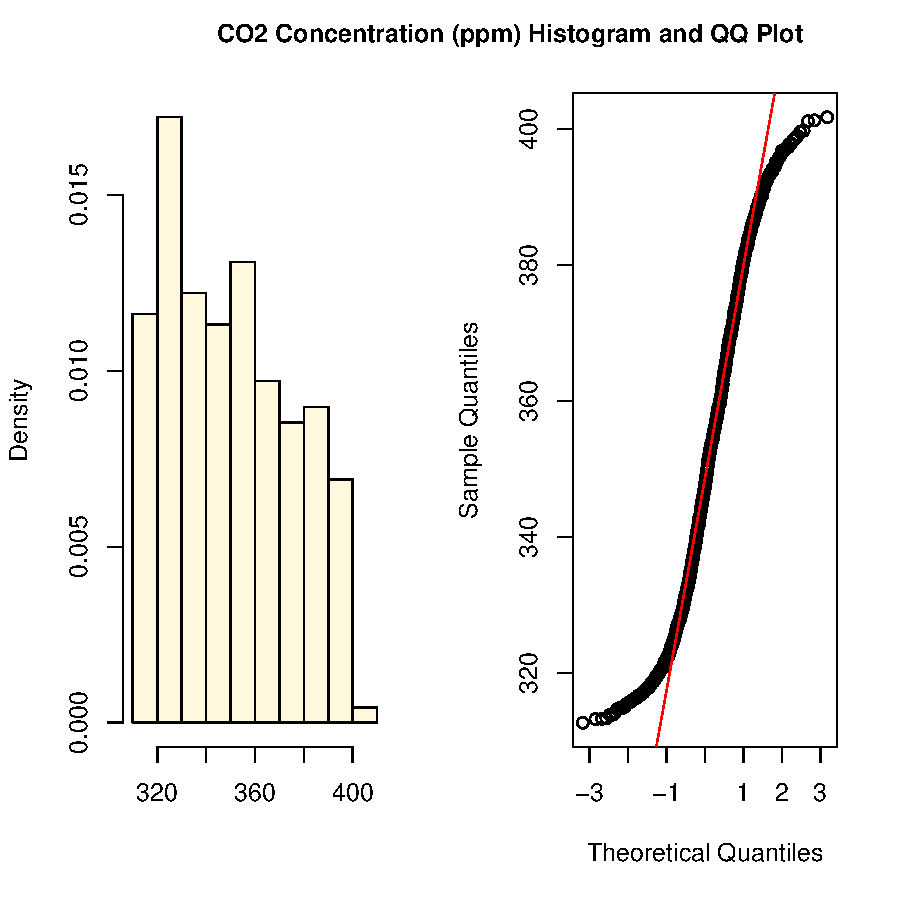
\includegraphics{alleselena-fig1check}


\subsubsection{Plotting the fitted values}
\begin{figure}[H]
\centering
\begin{Schunk}
\begin{Sinput}
> # Run a linear model
> datalm = lm( co2 ~ year)
> # Fit predict values
> MyData=data.frame(year=seq(from=(1958),to=2014, by=0.1))
> pred=predict(datalm, newdata=MyData, type="response", se=T)
> # Plot the fitted values
> plot(year, co2, type="n",las=1, xlab="Year", ylab="CO2 conc. (ppm)", 
      main="CO2 concentration in the atmosphere")
> grid (NULL,NULL, lty = 6, col = "cornsilk2")
> points(year, co2, col="cornflowerblue" )
> # Write confidence interval
> F=(pred$fit)
> FSUP=(pred$fit+1.96*pred$se.fit) # make upper conf. int.
> FSLOW=(pred$fit-1.96*pred$se.fit) # make lower conf. int.
> lines(MyData$year, F, lty=1, col="red", lwd=3)
> lines(MyData$year, FSUP,lty=1, col="red", lwd=3)
> lines(MyData$year, FSLOW,lty=1, col="red", lwd=3)
> legend("topleft",c("simple linear regression y~x", "monthly mean data"),
 pch=c(20,20), col=c("red", "cornflowerblue"))
\end{Sinput}
\end{Schunk}
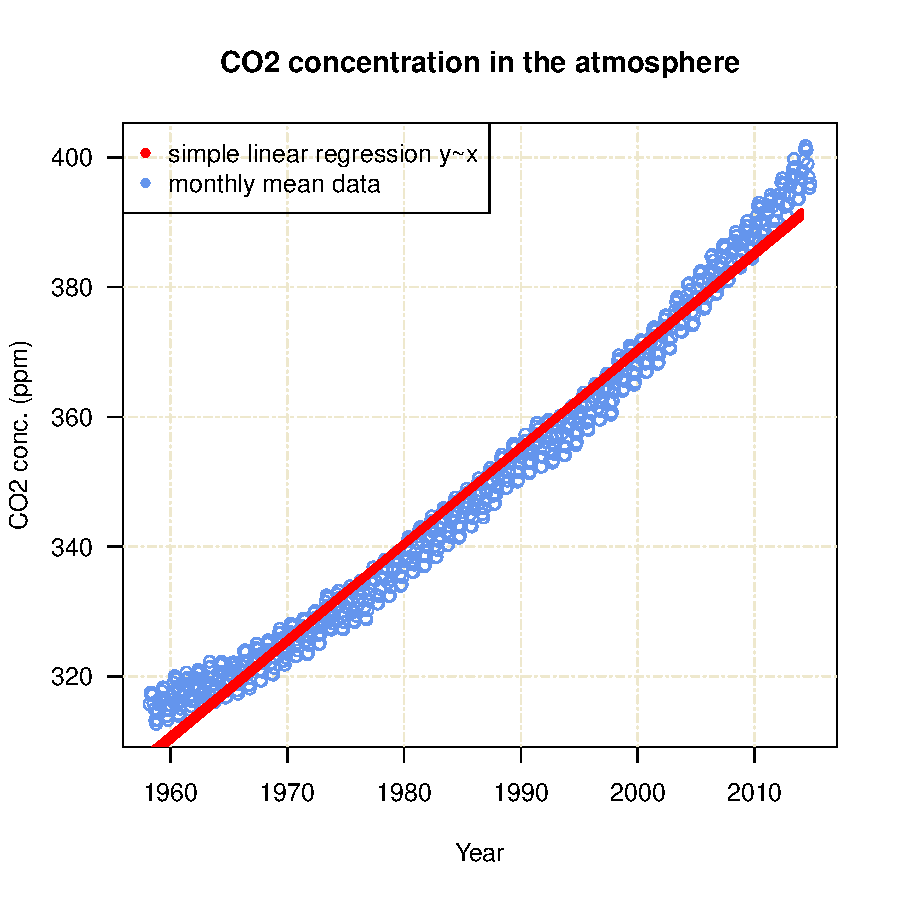
\includegraphics{alleselena-fig1datalm}
\end{figure}
Look at standard errors, highly underestimated, standard errors are higher in true ! p value is not right evidence , misleading :
\begin{Schunk}
\begin{Sinput}
> xtable(summary(datalm))
\end{Sinput}
% latex table generated in R 3.1.1 by xtable 1.7-4 package
% Wed Nov 26 19:43:21 2014
\begin{table}[ht]
\centering
\begin{tabular}{rrrrr}
  \hline
 & Estimate & Std. Error & t value & Pr($>$$|$t$|$) \\ 
  \hline
(Intercept) & -2618.5566 & 16.9782 & -154.23 & 0.0000 \\ 
  year & 1.4944 & 0.0085 & 174.86 & 0.0000 \\ 
   \hline
\end{tabular}
\end{table}\end{Schunk}
\noindent This plot (~\ref{fig1datalm} can be used to observe if there are outliers which could possibly bias the model. \\
However the poly-1 linear regression is not accurate in fitting the CO2-dataset. This is due to the present autocorrelation that not yet has been taken into account. Neglecting this factor will always effect the accuracy of the model results. The standard errors are lower than their true values thus giving high statistical significance with a p-value lower than it should be. The clue in statistical modelling is to present the correct statistical evidence, which would be highly biased with a linear model.\\
\subsection{Dataset Transformation}
It is essential to transform your dataset into a timeseries (ts) if you seek for an accurate and extensive analysis of the data.
\noindent The data stored as a dataframe needs to be transformed with the important columns into the class of a time series to continue working on it properly. If you have monthly data you have to set the deltat of the function ts() to deltat=1/12 describing the sampling period parts between successive values xt and xt+1. Your time series should somehow look like table 1.\\
\noindent \textbf{Original Data}\\
\begin{Schunk}
\begin{Sinput}
> xtable(head(data), caption="Original CO2-Data")
\end{Sinput}
% latex table generated in R 3.1.1 by xtable 1.7-4 package
% Wed Nov 26 19:43:21 2014
\begin{table}[ht]
\centering
\begin{tabular}{rrr}
  \hline
 & year & co2 \\ 
  \hline
1 & 1958.21 & 315.71 \\ 
  2 & 1958.29 & 317.45 \\ 
  3 & 1958.38 & 317.50 \\ 
  4 & 1958.46 & 317.10 \\ 
  5 & 1958.54 & 315.86 \\ 
  6 & 1958.62 & 314.93 \\ 
   \hline
\end{tabular}
\caption{Original CO2-Data} 
\end{table}\end{Schunk}
\noindent \textbf{Transformation}\\
\begin{Schunk}
\begin{Sinput}
> yourts=ts(co2, c(1958,3),c(2014,10), deltat=1/12)
> class(yourts)
\end{Sinput}
[1] "ts"\begin{Sinput}
> time = time(yourts)
> 
\end{Sinput}
\end{Schunk}
%<<results=tex, echo=FALSE, print=TRUE >>=
%print(xtable(yourts, digits=2, label="yourts",caption="Your time series for monthly mean data"), size="\\tiny")
%@
%\pagebreak
\subsection{Time-Series Visualization}%------------------------------------------------------------------------------------
It is important to get a quick overview of your data. Some simple plots for visualization are quite helpful.
\subsubsection{Time-Series Plot}
\begin{figure}[H]
\centering
\begin{Schunk}
\begin{Sinput}
> par(mfrow=c(1,1))
> plot.ts(yourts,las=1, xlab="Year", ylab="CO2 conc. (ppm)",
         main="CO2 concentration in the atmosphere")
> grid (NULL,NULL, lty = 6, col = "cornsilk2")
> points(yourts, col="cornflowerblue" )
> k <- 5
> lines(year,filter(co2, rep(1/k,k) ),col = 'red', type="l", lwd = 3)
> legend("topleft",c("simple moving average", "monthly mean data"),
 pch=c(20,20), col=c("red", "cornflowerblue"))
\end{Sinput}
\end{Schunk}
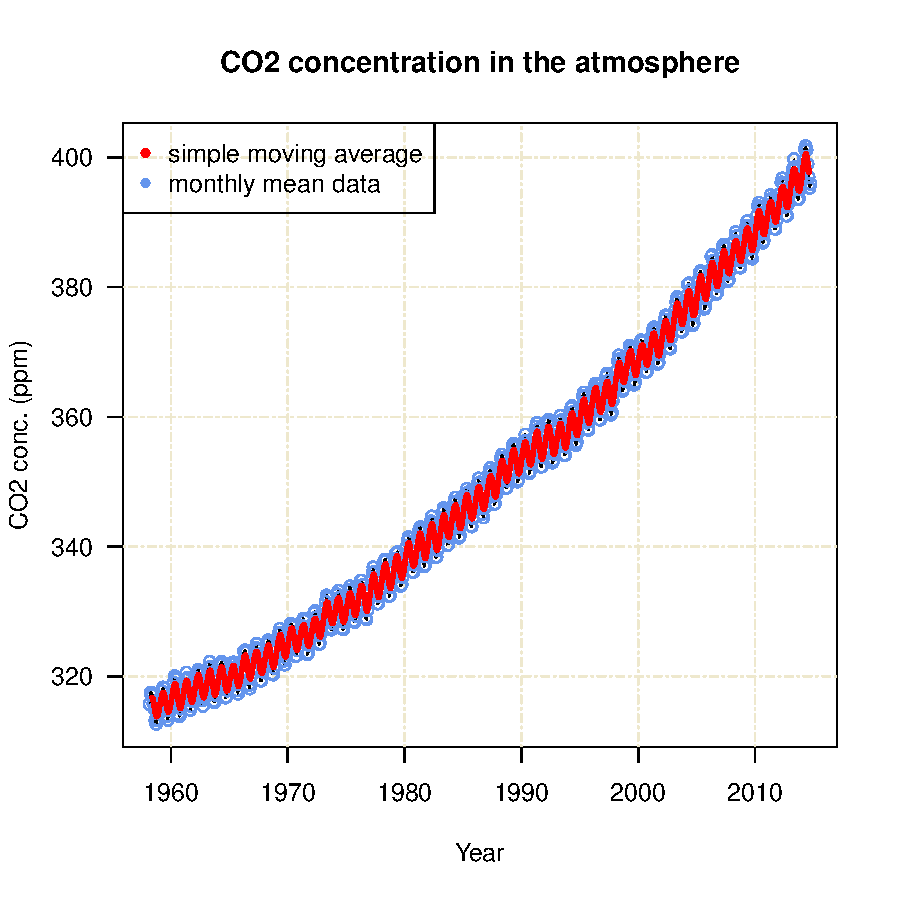
\includegraphics{alleselena-fig1visualize}
\caption{Visualization of the CO2 Concentrations}
\label{fig1visualize}
\end{figure}
\noindent \textbf{Note: The red line in plot \ref{fig1visualize} was computed with a simple moving average. It is not enough to just run a MA.}\\
%\pagebreak
\subsubsection{ACF, PACF, SPECTRUM}
\noindent Since time-series data usually violates the independence assumption of the model, the standard error is potentially too small. As the data are regularly spaced in time, we can easily employ the autocorrelation function to investigate residuals correlations in the model errors.\\
\textbf{The acf() function} can be used for that, which produces a plot of the correlogram.\\
Another nice procedure is to run the \textbf{autocorrelation function} with its complementary \textbf{partial acf} and the \textbf{spectrum} showing the spectral density of your time series at frequencies corresponding to the possibly approx. Fourier frequencies. \\

\begin{figure}[H]
\centering
\begin{Schunk}
\begin{Sinput}
> acf(co2, xlab="", main = "")
\end{Sinput}
\end{Schunk}
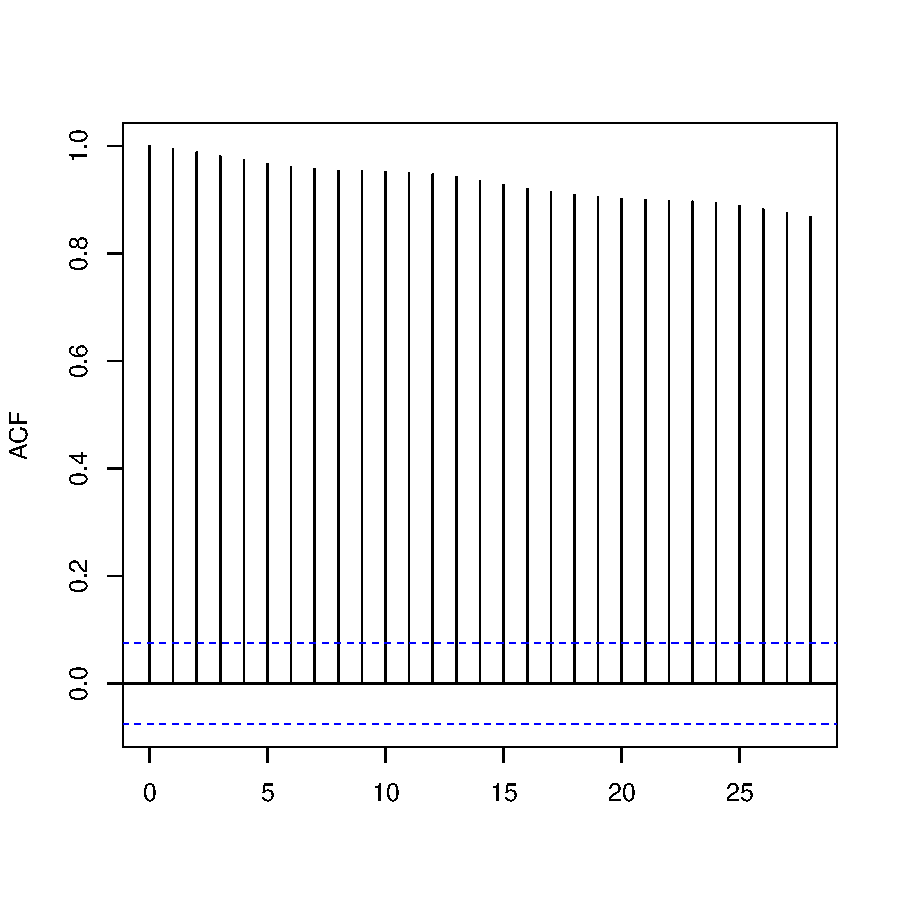
\includegraphics{alleselena-correlogramlm}
 \caption{ACF of CO2 Concentrations}
\label{correlogramlm}
\end{figure}


\begin{figure}[H]
\centering
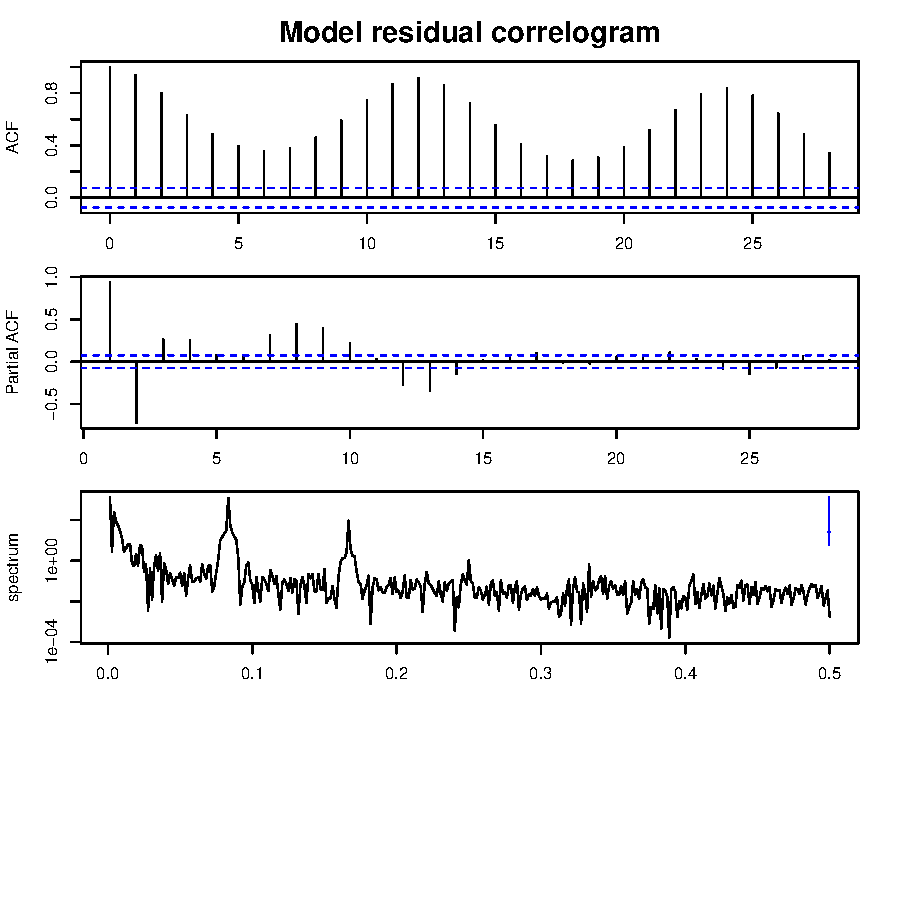
\includegraphics{alleselena-correlogramres}
\caption{Correlogram of residuals of lm}
\label{correlogramlm}
\end{figure}


Explain the acf , pacf, spectrum here. \\
\textbf{ACF \& PACF:}\\
\noindent The generated correlogram reveals that there are major autocorrelations. \\
There is a strong correlation at lag 1,a weaker correlation at lag 2, and a noticeable correlation at lag 3. Such a correlation pattern is typical for an autoregressive process where most of the sequential dependence can be explained as a flow-on effect from a dependence at lag 1.\\
\noindent In an autoregressive time series, an independent error component, or ''innovation" is associated with each time point. For an order p autoregressive time series, the error for any time point is obtained by taking the innovation for that time point, and adding a linear combination of the innovations at the p previous time points. (For the present time series, initial indications are that p = 1 might capture most of the correlation structure.)"\\ (autosmooth.pdf)\\
\noindent \textbf{Spectrum:} easier to interpret the acf / log scaled / strong cycles where spectrum max. occurs
Here the highest maximum is at about 0.75. 1/0.75 = 12 meaning a 12 month cycle is occuring here .\\
\noindent The residuals in a time series are serially correlated. The ACF is waving and decreases only slowly, which could be an identification of non-stationarity ( If the ACF would drop to zero quickly, the time series would be stationary). We stop all diagnostics here for our clearly wrong model and go on to investigate the different components of our time series.\\
\section{Decomposition of Time Series}%-----------------------------------------------------------------------------------------------------
A time serie consists of 3 components; a trend component, an irregular (random) component and (if it is a seosonal time series) seasonal component.
\subsection{Decomposing Seasonal Data}%----------------------------------------------------------------------------------------------------
\noindent We can decompose the ts and plot these components:
\begin{figure}[H]
\centering
\begin{Schunk}
\begin{Sinput}
> plot(decompose(yourts))
\end{Sinput}
\end{Schunk}
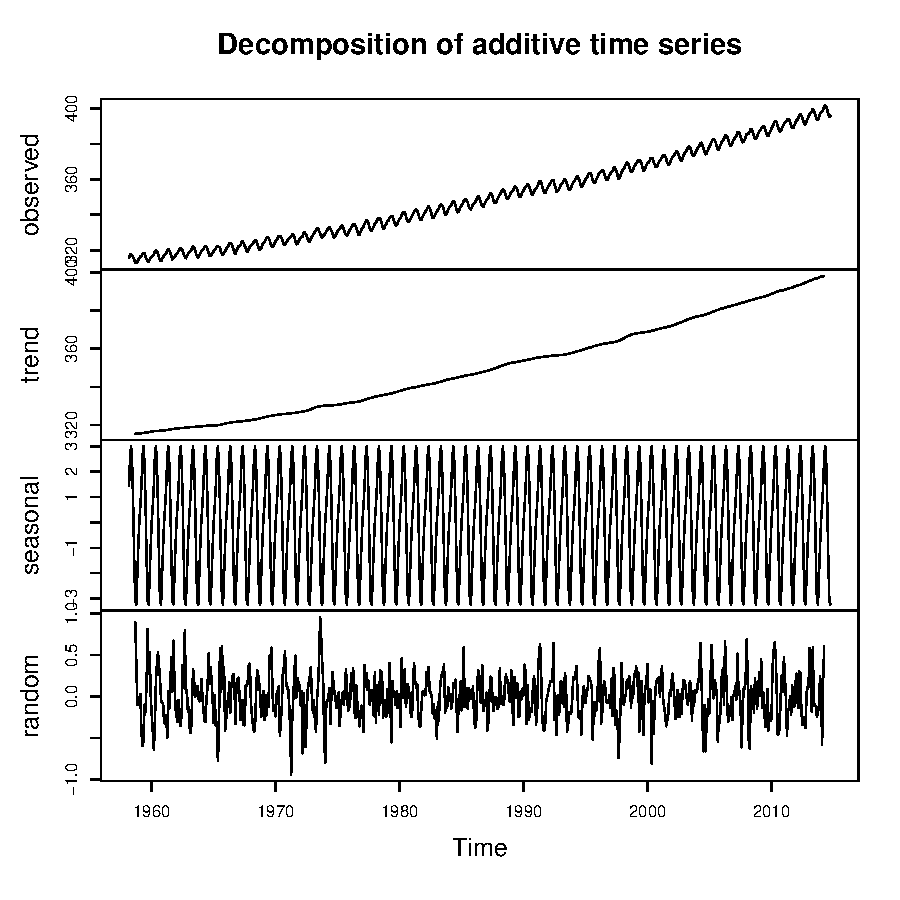
\includegraphics{alleselena-decompose}
\caption{Decomposition of the CO2 Time Series}
\end{figure}
\noindent We can see each component with:
\begin{Schunk}
\begin{Sinput}
> yourts_components<- decompose(yourts)
\end{Sinput}
\end{Schunk}
\begin{Schunk}
\begin{Sinput}
> yourts_components$seasonal
\end{Sinput}
\end{Schunk}
\begin{figure}[H]
\centering
\begin{Schunk}
\begin{Sinput}
> #we can see the trend for the first year:
> par(mfrow=c(1,2))
> ts.plot(yourts_components$seasonal[1:12])
> ts.plot(aggregate(yourts_components$seasonal))
\end{Sinput}
\end{Schunk}
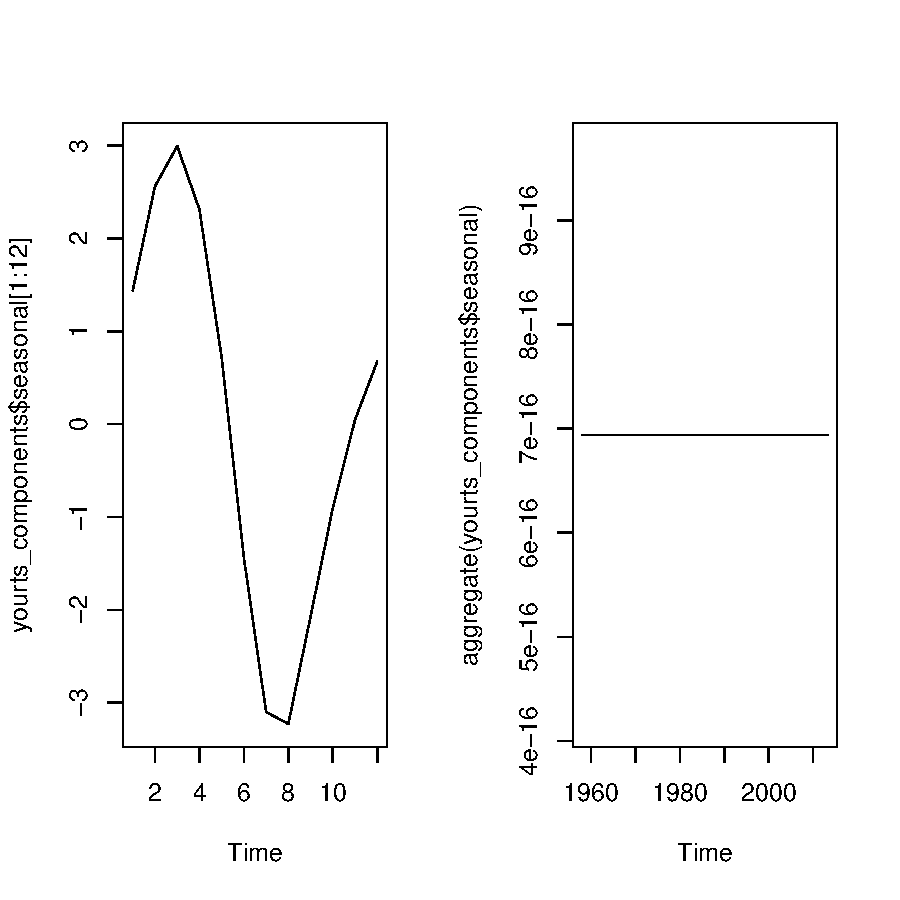
\includegraphics{alleselena-decomposition}
\caption{The seasonal component across the time}
\label{decomposition}
\end{figure}
It seems that our seasonal component is positive until the summer months, were it turns to be negative and turning to be positiv again in winter (see fig. ~\ref{decomposition}). And we can see in the right plot that this seasonal component is constant over all the years (see fig. ~\ref{decomposition}).
\begin{figure}[H]
\centering
\begin{Schunk}
\begin{Sinput}
> yourts_seasonallyadjusted <- yourts - yourts_components$seasonal
> par(mfrow=c(1,2))
> plot(yourts, main="TS with seasonal fl.", las=1)
> plot(yourts_seasonallyadjusted, las=1, main="removed seasonal fluctuation")
\end{Sinput}
\end{Schunk}
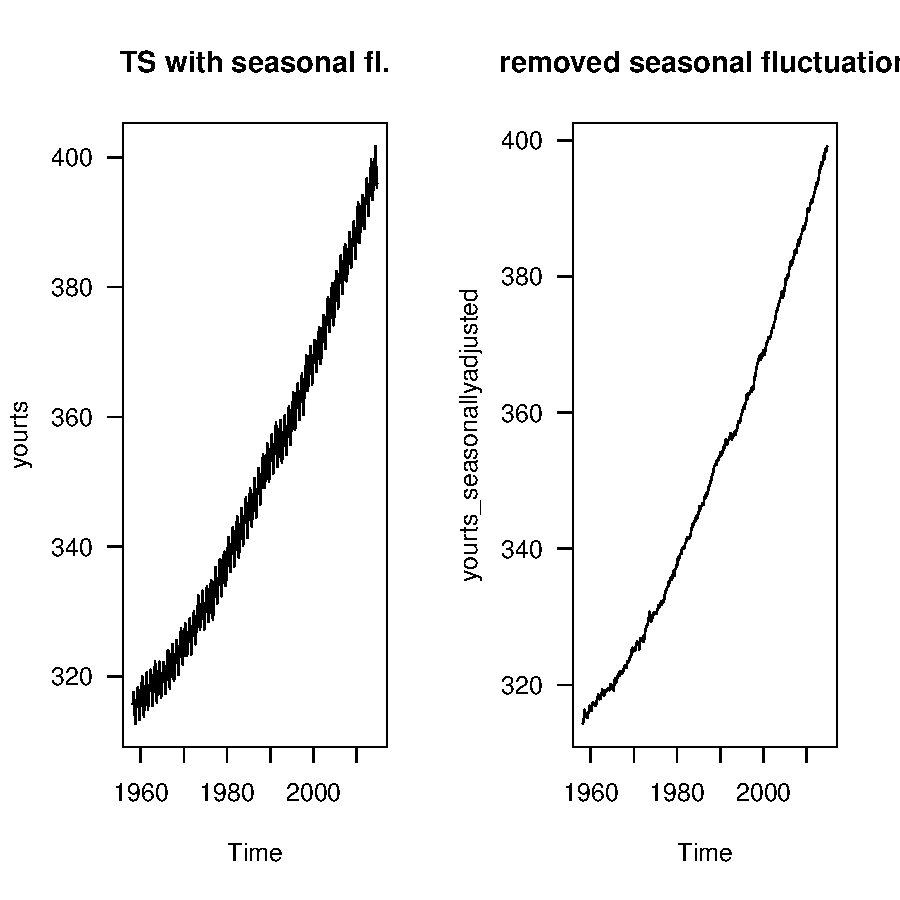
\includegraphics{alleselena-seasonallyadjusted}
\caption{Comparison of seasonal vs. seasonally adjusted model}
\label{decomposition2}
\end{figure}
\noindent It seems that our data can probably be described using an additive model, since the random fluctuations in the data are roughly constant in size over time (constant seasonal component). In some cases it might be handy to have the model without the seasonal fluctuations to depict change in the trend and local extremes easier (see fig. ~\ref{decomposition2}).

\section{Modelling the time series}
The best model for a time series needs to have residuals as white noise terms.
There are different ways to approach this task.

\subsection{Analysis of Seasonal Data with GLS}

GLS estimation:\\
If OLS is not optimal because of error term issues (as with serially correlated errors),
can often fix with Generalized Least Squares (GLS). GLS finds some transform of the original
model %so that the transformed model meets G-M assumptions, then do OLS on transformed
%model, untransform to get parameters of interest if necessary \\


##\\
\linebreak
After looking at the simple linear regression datalm, we were facing some serious problems with our model.
To be sure about non-stationarity of our time series, wen can run the adf.test, giving us the result that our data is non-stationary and we need to fix it:
\begin{Schunk}
\begin{Soutput}
	Augmented Dickey-Fuller Test

data:  yourts
Dickey-Fuller = -1.0663, Lag order = 8, p-value =
0.928
alternative hypothesis: stationary
\end{Soutput}
\end{Schunk}
Also we need a model which is covering the serial correlation of our residuals. The ACF, PACF, spectrum above gives us certainty an the autocorrelation and the seasonality.
The standard errors are highly underestimated, thus in the summary the p-value is too small and misleading.
A nice model to try is GLS, which will allow for correlation of standard errors and unequel variances.
In the GLS we have different options to choose, though our data is not spatially correlated we are not discussing spatial autocorrelation here ( further reading on:...)
Our first try on gls will be simple:
\begin{Schunk}
\begin{Sinput}
> data.glsAR = gls(yourts ~ time,cor= corAR1(acf(resid(datalm))$acf[2]))
> save(data.glsAR, file="data.glsAR.RData")
\end{Sinput}
\end{Schunk}

\begin{Schunk}
\begin{Sinput}
> load("data.glsAR.RData")
\end{Sinput}
\end{Schunk}

The difference will be made in the correlation structure. There are generally ( for temporal corr. interesting) five options you have:
\begin{enumerate}
\item corAR1: in ACF exponential decreasing values of correlation with time distance\\
\item corARMA: either autoregressive order or moving average order or both\\
\item corCAR1: continuous time ( time index does nto have to be integers)\\
\item corCompSymm: correlation does not decrease with higher distance\\
\item corSymm: general correlation only for few observations only, often overparameterized\\
\end{enumerate}
Our first gls model accounts for the AR1, which is clearly visible in the PACF.

\begin{figure}[H]
\centering
\begin{Schunk}
\begin{Sinput}
> par(mfrow=c(1,2))
> acf(data.glsAR$residuals)
> pacf(data.glsAR$residuals)
\end{Sinput}
\end{Schunk}
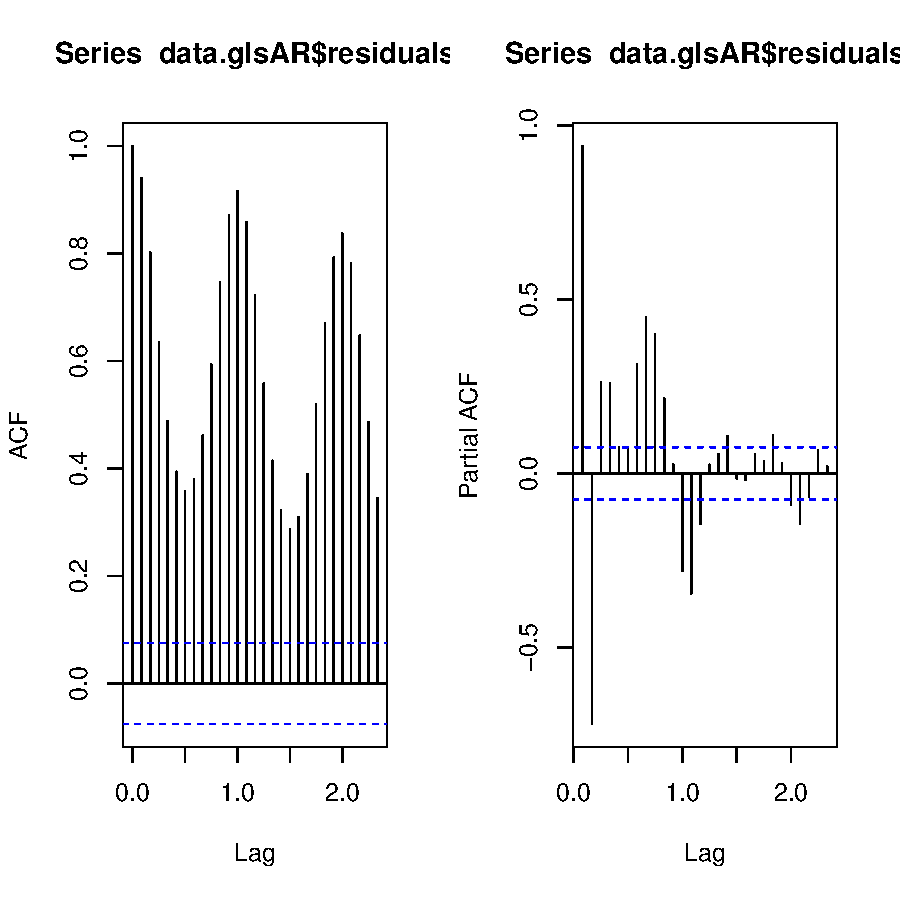
\includegraphics{alleselena-correlogram}
\caption{Correlogram of GLS  with AR(1) structure}
\label{corglsAR}
\end{figure}

We have still a lot of problems concerning the autocorrelation and the seasonality. One option is to allow the AR to use more parameters and/or to include a moving average or error variance to the model. This can be handled via the corARMA. We tried 2 versions, one with 1 lag and 1 moving average, the other with 2 lags and 2 moving averages.
The 0.2 are starting values for Phi, which are in the modelling process optimized.
The next models are thus:
\begin{Schunk}
\begin{Sinput}
> data.glsARMA1 = gls ( yourts ~ time, cor = corARMA (c(0.2,0.2),p=1, q=1 ))
> data.glsARMA2 = gls ( yourts ~ time, cor=corARMA(c(0.2,0.2,0.2,0.2), p=2, q=2))
> save(data.glsARMA1, file="data.glsARMA1.RData")
> save(data.glsARMA2, file="data.glsARMA2.RData")
\end{Sinput}
\end{Schunk}

\begin{Schunk}
\begin{Sinput}
> load("data.glsARMA1.RData")
> load("data.glsARMA2.RData")
\end{Sinput}
\end{Schunk}

To compare all the models we use anova and the best model is so far the data.glsARMA2 with the lowest AIC and significantly better than the ARMA1, which is itself significantly better than the data.glsAR.
\begin{Schunk}
\begin{Sinput}
>  #run diagnostics
> diagnostics(data.glsARMA2)
\end{Sinput}
\begin{Soutput}
$`norm. distrb. of residuals`

	Shapiro-Wilk normality test

data:  x$residuals
W = 0.9785, p-value = 1.863e-08


$`stationarity of residuals`

	Augmented Dickey-Fuller Test

data:  x$residuals
Dickey-Fuller = -1.0663, Lag order = 8, p-value =
0.928
alternative hypothesis: stationary


$`stationarity of fitted values`

	Augmented Dickey-Fuller Test

data:  x$fitted
Dickey-Fuller = 0.0492, Lag order = 8, p-value = 0.99
alternative hypothesis: stationary


$`autocorrelation of residuals`
[1] 0.1111867

$`independence of residuals`

	Box-Ljung test

data:  x$residuals
X-squared = 603.775, df = 1, p-value < 2.2e-16
\end{Soutput}
\begin{Sinput}
> 
\end{Sinput}
\end{Schunk}

\begin{figure}[H]
\centering
\begin{Schunk}
\begin{Sinput}
> plot(datalm, which = 1:1)
> #well spread is already smaller of variances
\end{Sinput}
\end{Schunk}
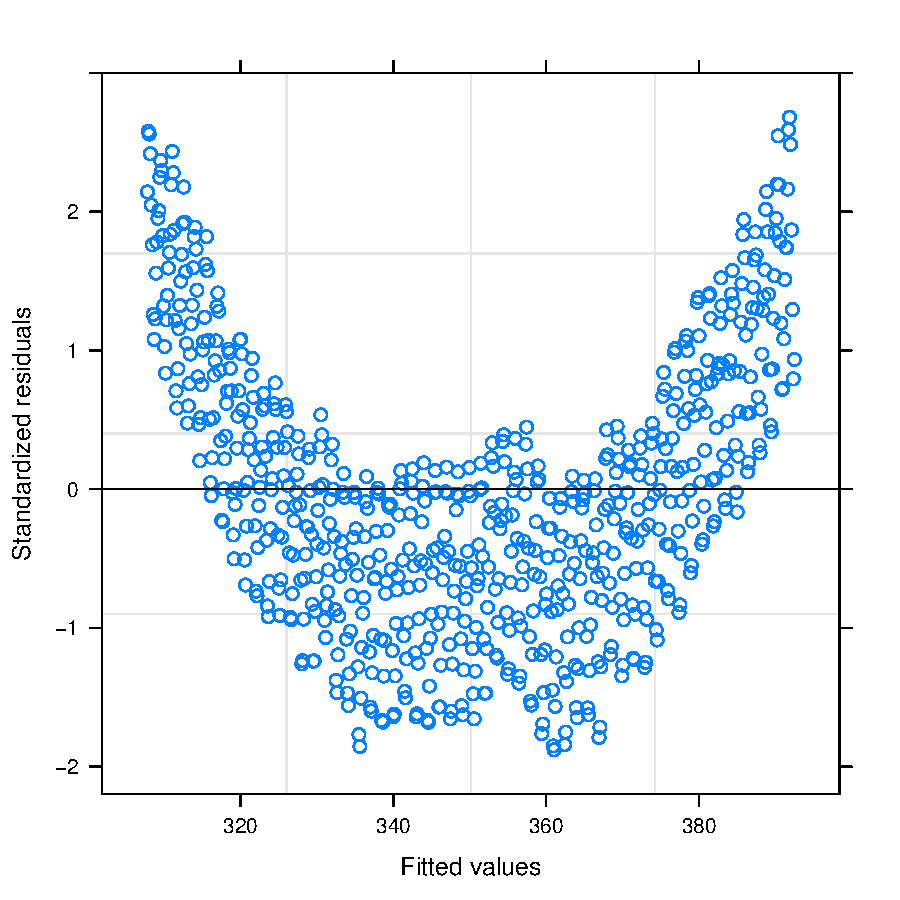
\includegraphics{alleselena-residual}
\caption{Residuals fitted vs. observed in LM}
\label{residual}
\end{figure}\\

\begin{figure}[H]
\centering
\begin{Schunk}
\begin{Sinput}
> plot(data.glsARMA2)
\end{Sinput}
\end{Schunk}
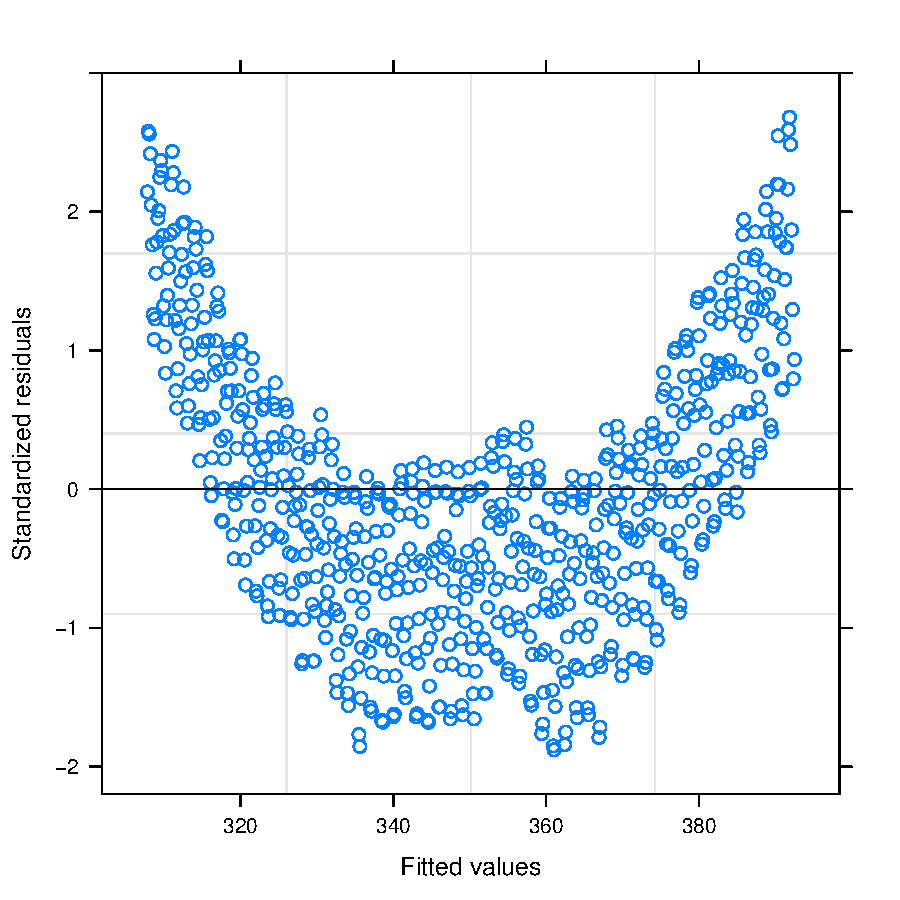
\includegraphics{alleselena-residual}
\caption{Residuals fitted vs. observed in GLS}
\label{residual}
\end{figure}\\

\noindent function writing: if anovaAIC lowest, choose this as bestmodel
But still we have seasonal problems here. We should therefore include a seasonal term.
Try to fit for seasonal component and autocorrelation with best corstruct:

\begin{Schunk}
\begin{Sinput}
> seas = cycle(yourts)
> dataseasongls = gls(yourts ~ time + factor(seas), cor=corARMA( c(0.2,0.2,0.2, 0.2),
                 p=2, q=2)) #use bestmodel corStruct
> save(dataseasongls, file="dataseasongls.RData")
\end{Sinput}
\end{Schunk}

\begin{Schunk}
\begin{Sinput}
> load("dataseasongls.RData")
\end{Sinput}
\end{Schunk}

\begin{figure}[H]
\centering
\begin{Schunk}
\begin{Sinput}
> par(mfrow=c(2,1))
> acf(dataseasongls$residuals)
> pacf(dataseasongls$residuals)
\end{Sinput}
\end{Schunk}
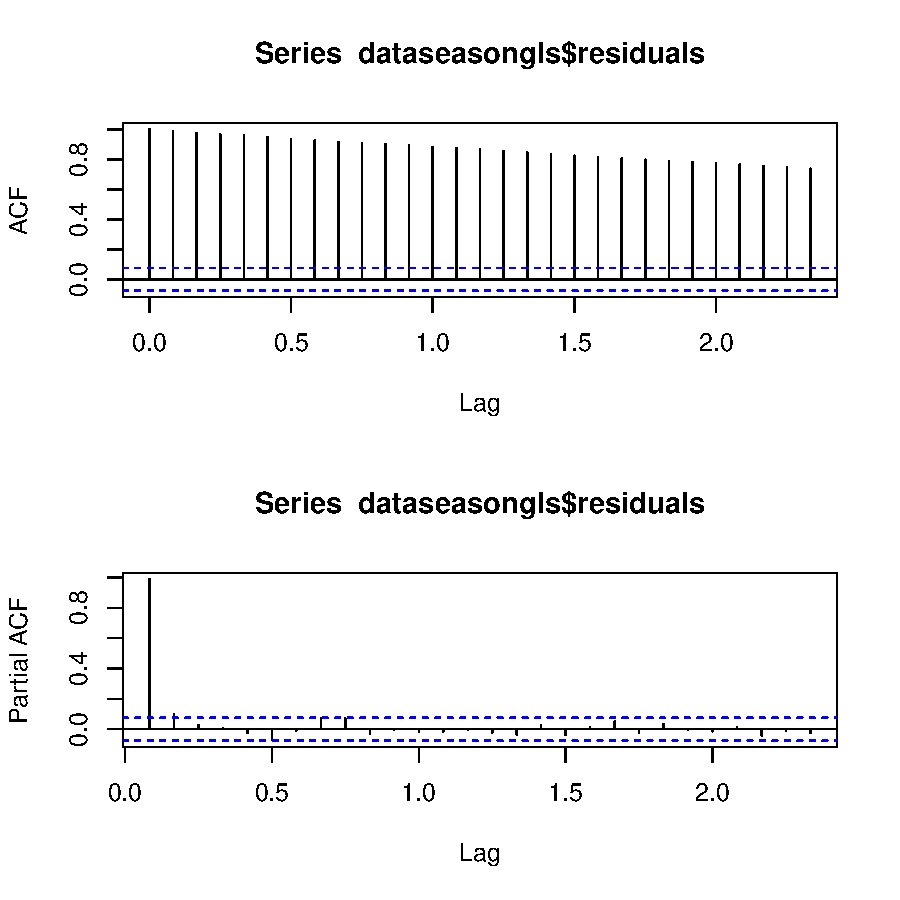
\includegraphics{alleselena-corseas}
\caption{Correlogram of season included model}
\label{corseas}
\end{figure}


\begin{figure}[H]
\centering
\begin{Schunk}
\begin{Sinput}
> par(mfrow=c(1,1))
> ts.plot(dataseasongls$residuals) 
> #puuhh gar nich mal soo gut
\end{Sinput}
\end{Schunk}
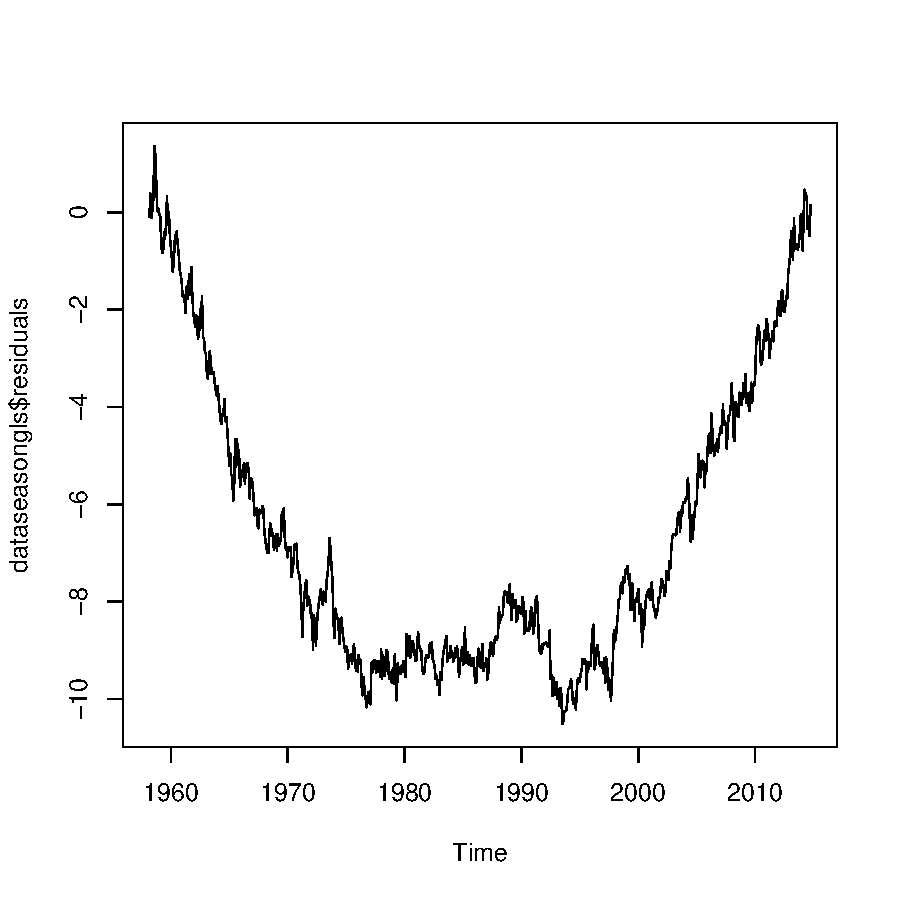
\includegraphics{alleselena-resseas}
\caption{Residuals of season included model}
\label{resseas}
\end{figure}

#print(anova(data.glsAR, data.glsARMA1, data.glsARMA2, dataseasongls))
oh boy cannot compare gls with different fixed effects, REML comparisons not meaningful, added a fixed effect: factor(seas)
so, maybe just look at AIC separately 

##AIC #smallest value best value = best model (trade off blabla)

\begin{Schunk}
\begin{Sinput}
> AIC(data.glsARMA2)
\end{Sinput}
[1] 1495.348\begin{Sinput}
> AIC(dataseasongls)
\end{Sinput}
[1] 401.2934\begin{Sinput}
> #write function choosing best model 
\end{Sinput}
\end{Schunk}

\begin{figure}[H]
\centering
\begin{Schunk}
\begin{Sinput}
> ts.plot(cbind(yourts, data.glsARMA2$fitted,dataseasongls$fitted),
         lty=1:2, col=c(1,2,3), main="Compare mean monthly data with gls model")
> legend(1960,400,c("Original", "Fitted for Autocorrelation","Fitted for Seasonality"),
        col=c(1,2,3),lty=c(1, 2,3))
\end{Sinput}
\end{Schunk}
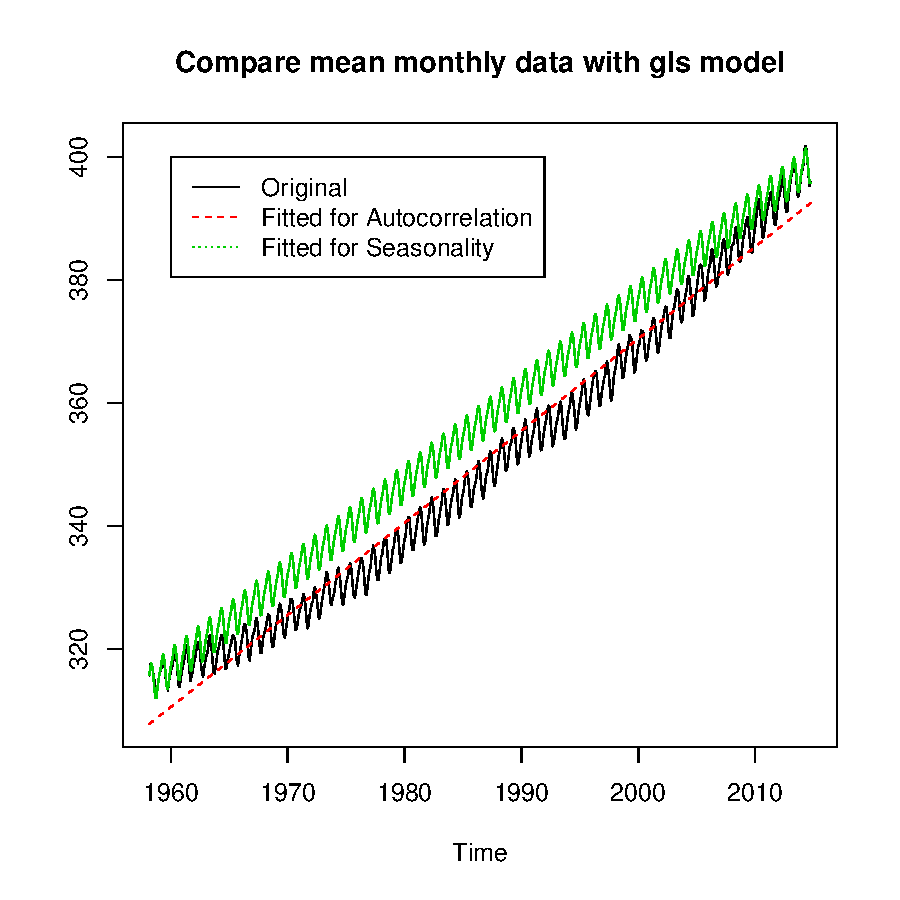
\includegraphics{alleselena-036}
\caption{Comparison of season included model and only autocorr. included model}
\label{compseas}
\end{figure}

In the figure ~\ref{compseas} you see the options we were trying so far to come closer to our adequate model. One option is the ARMA2 GLS including autocorrelation, the second option is to include the seasonality and adding a fixed effect ( factor(season)) to our gls. 
The seasonal effect inclusion clearly improves our model. But the original data is slightly curved. \\

We should include a quadratic term and generalize our seasonality with a continuous sin-cos wave:\\

\begin{Schunk}
\begin{Sinput}
> SIN = COS = matrix(nr=length(yourts), nc=6)
> for (i in 1:6) {
   COS[,i] <- cos(2*pi*i*time(yourts))
   SIN[,i] <- sin(2*pi*i*time(yourts)) 
 }
> time = time(yourts)
\end{Sinput}
\end{Schunk}
#also was done by hand in self writing seasonality removal above
Thus we do not know how many changes in the wave we need to include, we include 6 changes in the wave to be certain that the next model can follow the best wave option. 

Before this, add a quadratic term ( polynomial (x,2)), x = years) will change the linear regression by including a slight bending in the fitted values over time, which we saw in the original data. 

\begin{Schunk}
\begin{Sinput}
> harmonizedgls<-gls(yourts ~ time + I(time^2) +
                     COS[,1]+SIN[,1]+COS[,2]+SIN[,2]+
                     COS[,3]+SIN[,3]+COS[,4]+SIN[,4]+
                     COS[,5]+SIN[,5]+COS[,6]+SIN[,6],
                   corr=corAR1(acf(dataseasongls$residuals)$acf[2]))
> save(harmonizedgls, file="harmonizedgls.RData")
> harmonizedARMAgls<-gls(yourts ~ time + I(time^2) +
                       COS[,1]+SIN[,1]+COS[,2]+SIN[,2]+
                       COS[,3]+SIN[,3]+COS[,4]+SIN[,4]+
                       COS[,5]+SIN[,5]+COS[,6]+SIN[,6]
                     , cor=corARMA(p=2, q=2))
> save(harmonizedARMAgls, file="harmonizedARMAgls.RData")
\end{Sinput}
\end{Schunk}

\begin{Schunk}
\begin{Sinput}
> load("harmonizedARMAgls.RData")
> load("harmonizedgls.RData")
\end{Sinput}
\end{Schunk}

\begin{Schunk}
\begin{Sinput}
> AIC(harmonizedgls) #even smaller 
\end{Sinput}
\begin{Soutput}
[1] 396.86
\end{Soutput}
\begin{Sinput}
> AIC(harmonizedARMAgls) #even smaller 
\end{Sinput}
\begin{Soutput}
[1] 360.4082
\end{Soutput}
\begin{Sinput}
> xtable(anova(harmonizedgls,harmonizedARMAgls))
\end{Sinput}
\begin{Soutput}
% latex table generated in R 3.1.1 by xtable 1.7-4 package
% Wed Nov 26 19:43:23 2014
\begin{table}[ht]
\centering
\begin{tabular}{rlrrrrrlrr}
  \hline
 & call & Model & df & AIC & BIC & logLik & Test & L.Ratio & p-value \\ 
  \hline
harmonizedgls & gls(model = yourts \~{} time + I(time\verb|^|2) + COS[, 1] + SIN[, 1] +     COS[, 2] + SIN[, 2] + COS[, 3] + SIN[, 3] + COS[, 4] + SIN[,     4] + COS[, 5] + SIN[, 5] + COS[, 6] + SIN[, 6], correlation = corAR1(acf(dataseasongls\$residuals)\$acf[2])) &   1 &  17 & 396.86 & 473.36 & -181.43 &  &  &  \\ 
  harmonizedARMAgls & gls(model = yourts \~{} time + I(time\verb|^|2) + COS[, 1] + SIN[, 1] +     COS[, 2] + SIN[, 2] + COS[, 3] + SIN[, 3] + COS[, 4] + SIN[,     4] + COS[, 5] + SIN[, 5] + COS[, 6] + SIN[, 6], correlation = corARMA(p = 2,     q = 2)) &   2 &  20 & 360.41 & 450.40 & -160.20 & 1 vs 2 & 42.45 & 0.00 \\ 
   \hline
\end{tabular}
\end{table}
\end{Soutput}
\end{Schunk}
tja das mit der xtable print(xtable) is alles eher s...uppressiv f<fc>r mein Hirn. \\

\begin{figure}[H]
\centering
\begin{Schunk}
\begin{Sinput}
> par(mfrow=c(1,1))
> ts.plot(cbind(yourts,harmonizedARMAgls$fitted), col=c(1,3),
         main="Compare mean monthly data with gls model")
> legend(1960,400,c("Original", "Included seasonality ",
                   "Polynm. + seasonality"),col=c(1,2,3), pch=c(20,20,20))
\end{Sinput}
\end{Schunk}
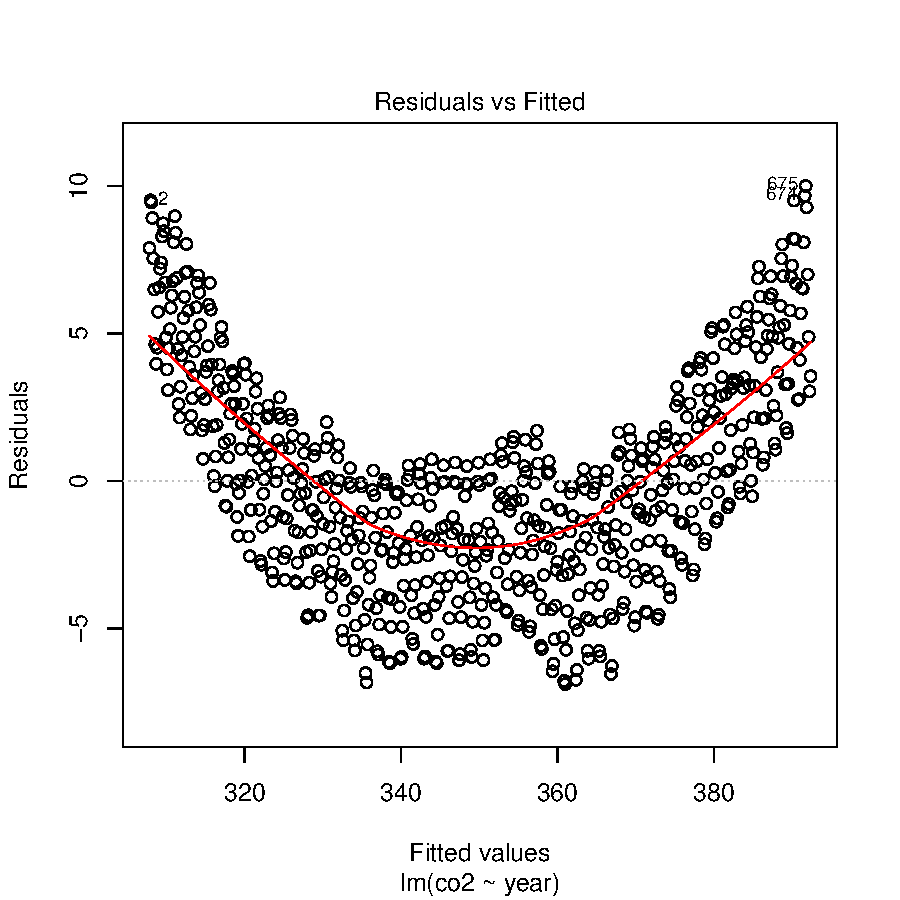
\includegraphics{alleselena-042}
\caption{Comparison of season and quadr. term included model}
\label{compq}
\end{figure}

\linebreak
residuals compare\\
\begin{figure}[H]
\centering
\begin{Schunk}
\begin{Sinput}
> plot(datalm, which = 1:1)
\end{Sinput}
\end{Schunk}
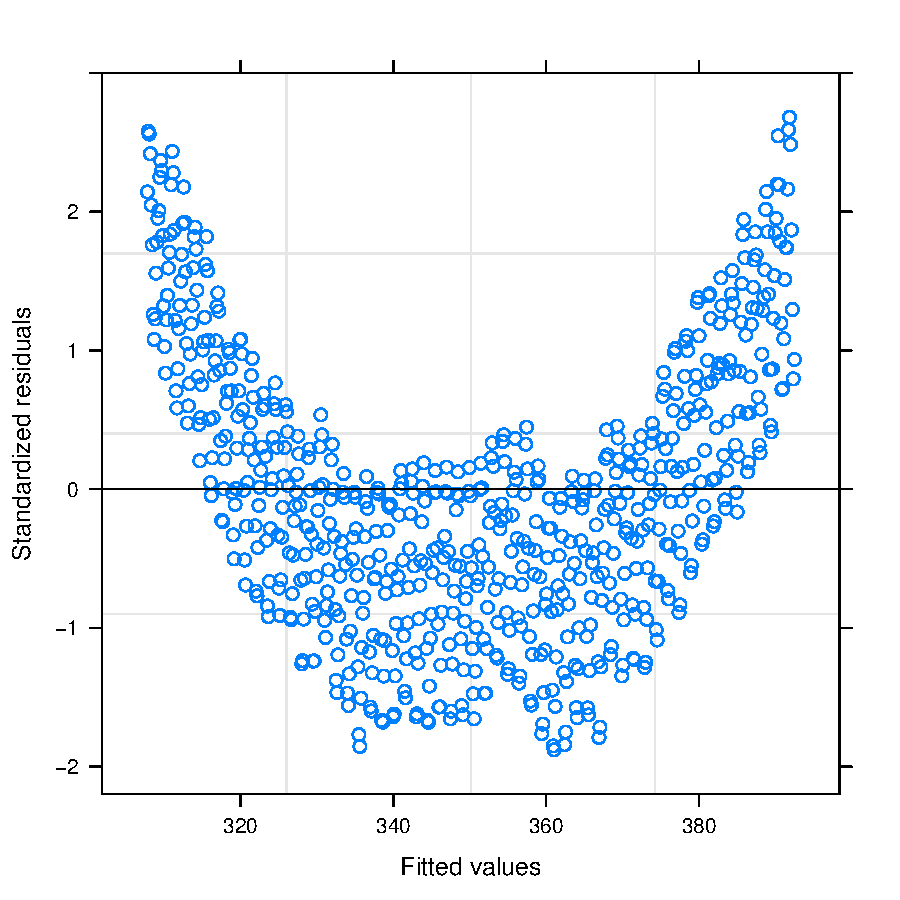
\includegraphics{alleselena-043}
\caption{Residuals fitted vs. obs. values}
\label{comparison_finalgls1}
\end{figure}

\begin{figure}[H]
\centering
\begin{Schunk}
\begin{Sinput}
> plot(data.glsARMA2)
\end{Sinput}
\end{Schunk}
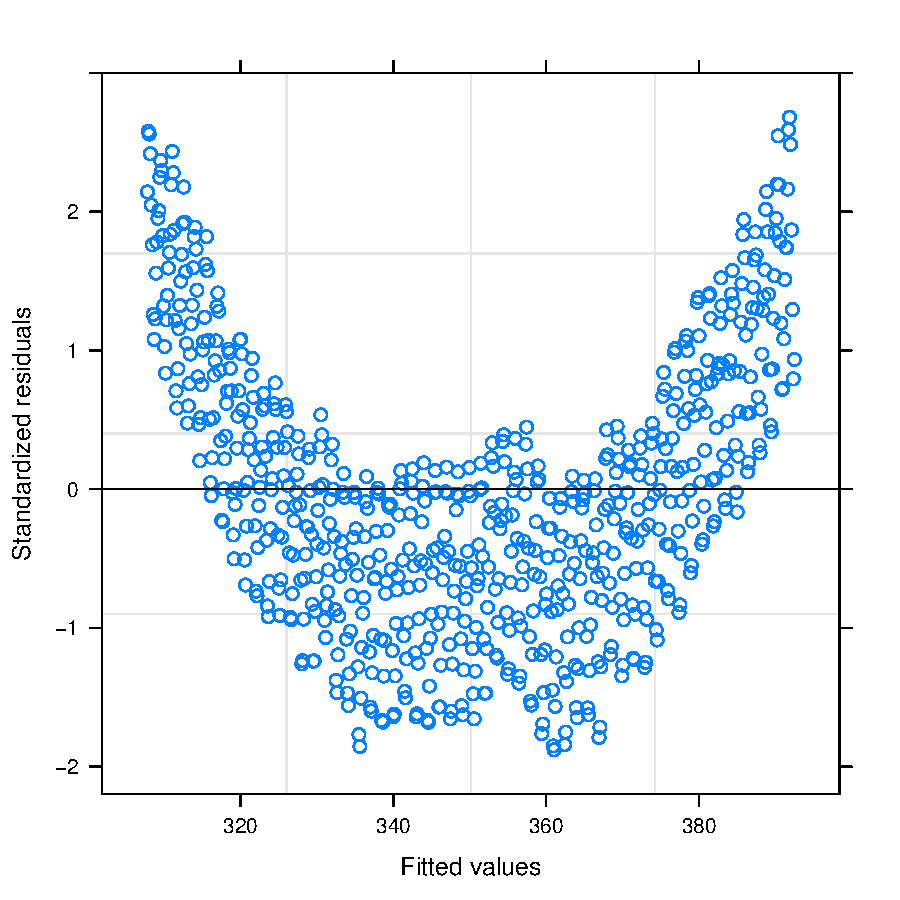
\includegraphics{alleselena-044}
\caption{Residuals fitted vs. obs. values ARMA}
\label{comparison_finalgls2}
\end{figure}

\begin{figure}[H]
\centering
\begin{Schunk}
\begin{Sinput}
> plot(harmonizedARMAgls)
\end{Sinput}
\end{Schunk}
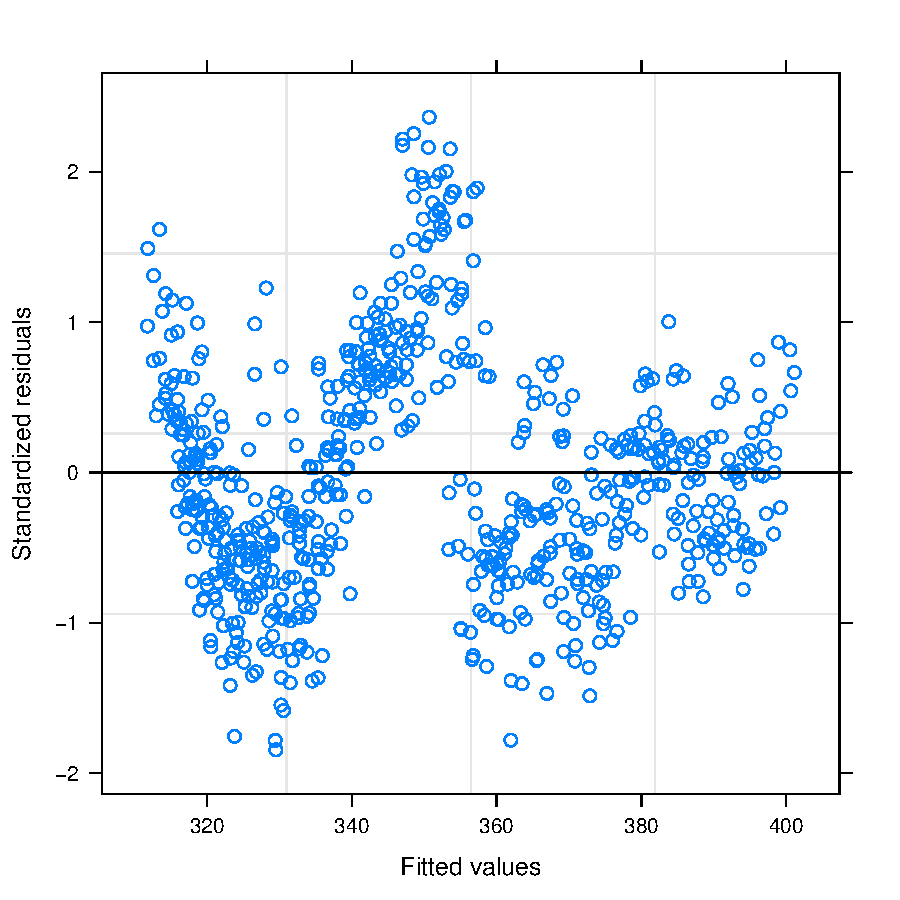
\includegraphics{alleselena-045}
\caption{Residuals fitted vs. obs. values ARMA harm.}
\label{comparison_finalgls3}
\end{figure}

\begin{Schunk}
\begin{Sinput}
> list = as.list(diagnostics(harmonizedARMAgls))
> print(list)
\end{Sinput}
\begin{Soutput}
$`norm. distrb. of residuals`

	Shapiro-Wilk normality test

data:  x$residuals
W = 0.98, p-value = 5.229e-08


$`stationarity of residuals`

	Augmented Dickey-Fuller Test

data:  x$residuals
Dickey-Fuller = -2.6803, Lag order = 8, p-value =
0.2904
alternative hypothesis: stationary


$`stationarity of fitted values`

	Augmented Dickey-Fuller Test

data:  x$fitted
Dickey-Fuller = -0.4144, Lag order = 8, p-value =
0.9857
alternative hypothesis: stationary


$`autocorrelation of residuals`
[1] 0.183333

$`independence of residuals`

	Box-Ljung test

data:  x$residuals
X-squared = 563.3192, df = 1, p-value < 2.2e-16
\end{Soutput}
\end{Schunk}

\begin{figure}[H]
\centering
\begin{Schunk}
\begin{Sinput}
> qqnorm(harmonizedARMAgls, abline=c(0,1))
\end{Sinput}
\end{Schunk}
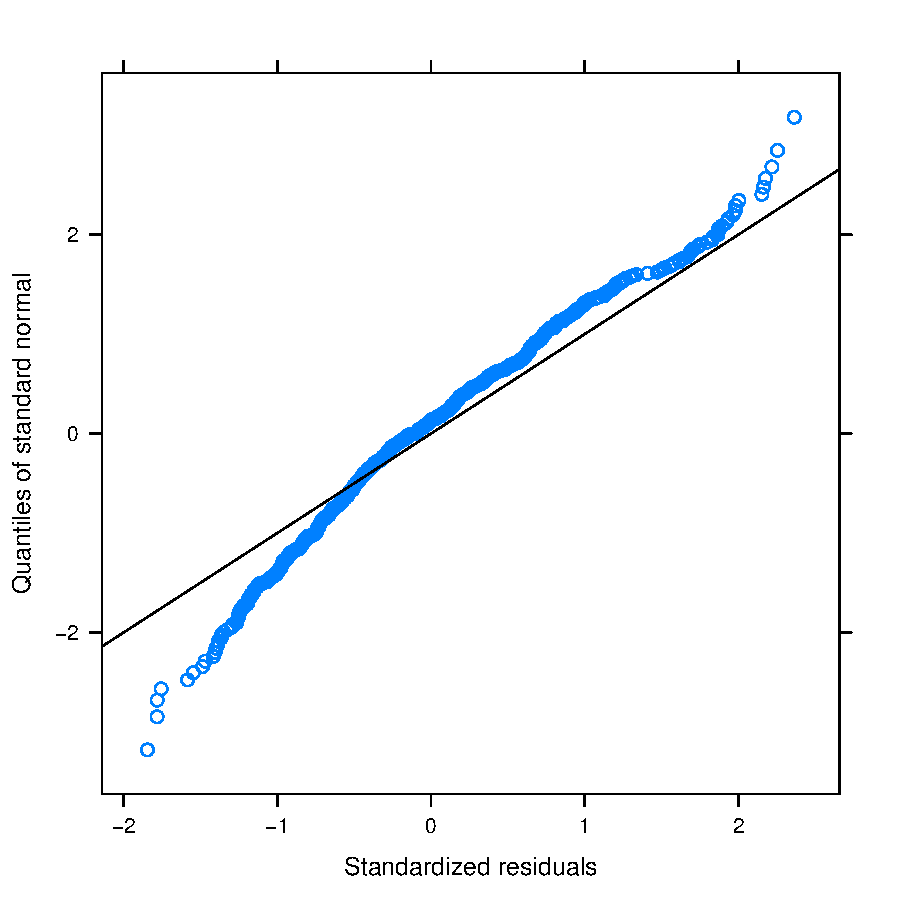
\includegraphics{alleselena-047}
\caption{look at norm. distribution}
\label{finalgls_norm}
\end{figure}

\linebreak
#bestmodel with smallest AIC: \\
\begin{Schunk}
\begin{Sinput}
> anova.all = anova( harmonizedgls,harmonizedARMAgls)
> #as.matrix(anova.all)
> bestmodel= anova.all$Model[anova.all$AIC ==min(anova.all$AIC)]
> bestmodel 
\end{Sinput}
\begin{Soutput}
[1] 2
\end{Soutput}
\begin{Sinput}
> #Our best model fitted by hand is the model: \Sexpr{bestmodel} ...
\end{Sinput}
\end{Schunk}

\begin{table}[ht]
\centering
\begin{tabular}{rlrrrrrlrr}
  \hline
 Model & df & AIC & BIC & logLik & Test & L.Ratio & p-value \\ 
  \hline
harmonizedgls  &    17 & 396.86 & 473.36 & -181.43 &  &  &  \\ 
  harmonizedARMAgls  &    20 & 360.41 & 450.40 & -160.20 & 1 vs 2 & 42.45 & 3.21739e$-$09 \\ 
   \hline
\end{tabular}
\end{table}

\linebreak

compare standard errors: 
\begin{Schunk}
\begin{Sinput}
> sqrt(diag(vcov(datalm)))
\end{Sinput}
 (Intercept)         year 
16.978232786  0.008546518 \begin{Sinput}
> sqrt(diag(vcov(data.glsARMA2)))
\end{Sinput}
(Intercept)        time 
45.70868380  0.02300935 \begin{Sinput}
> sqrt(diag(vcov(harmonizedARMAgls))[c(1,2,3)])
\end{Sinput}
 (Intercept)         time    I(time^2) 
4.322027e+03 4.351766e+00 1.095347e-03 \end{Schunk}
\linebreak
#you see now the estimated errors are not underestimated anymore, 


\linebreak

  yes this was the gls 
#there are still some diagnostics failed! 
#non normally distributed - could normalize the residuals ? 
#not independent - not important for our models used
#but the autocorrelation was solved
#and the model is now stationary 

\subsection{Modelling time series with ARIMA }
First good thing: ARIMA does not care about stationarity. If your dataset is non-stationary, it will make it stationary as good as possible. auto.arima() gives me perfect adjusted time series model with trend, seasonal component and random terms.\\


\begin{Schunk}
\begin{Sinput}
> autoarima = auto.arima(yourts)
\end{Sinput}
Series: yourts 
ARIMA(1,1,1)(2,1,2)[12]                    

Coefficients:
         ar1      ma1     sar1     sar2     sma1     sma2
      0.2166  -0.5763  -0.2861  -0.0364  -0.5992  -0.2292
s.e.  0.0936   0.0782      NaN   0.0404      NaN      NaN

sigma^2 estimated as 0.08927:  log likelihood=-149.46
AIC=312.92   AICc=313.09   BIC=344.44\begin{Sinput}
> print(autoarima)
\end{Sinput}
Series: yourts 
ARIMA(1,1,1)(2,1,2)[12]                    

Coefficients:
         ar1      ma1     sar1     sar2     sma1     sma2
      0.2166  -0.5763  -0.2861  -0.0364  -0.5992  -0.2292
s.e.  0.0936   0.0782      NaN   0.0404      NaN      NaN

sigma^2 estimated as 0.08927:  log likelihood=-149.46
AIC=312.92   AICc=313.09   BIC=344.44
Series: yourts 
ARIMA(1,1,1)(2,1,2)[12]                    

Coefficients:
         ar1      ma1     sar1     sar2     sma1     sma2
      0.2166  -0.5763  -0.2861  -0.0364  -0.5992  -0.2292
s.e.  0.0936   0.0782      NaN   0.0404      NaN      NaN

sigma^2 estimated as 0.08927:  log likelihood=-149.46
AIC=312.92   AICc=313.09   BIC=344.44\end{Schunk}

\begin{figure}[H]
\centering
\begin{Schunk}
\begin{Sinput}
> fitted=fitted(autoarima)
> par(mfrow=c(1,1))
> ts.plot(cbind(yourts, harmonizedARMAgls$fitted), col=c(1,2))
> lines( fitted, col=3)
> legend(1960,400,c("Original",  "GLS", "Autoarima "),col=c(1,2,3), pch=c(20,20,20))
\end{Sinput}
\end{Schunk}
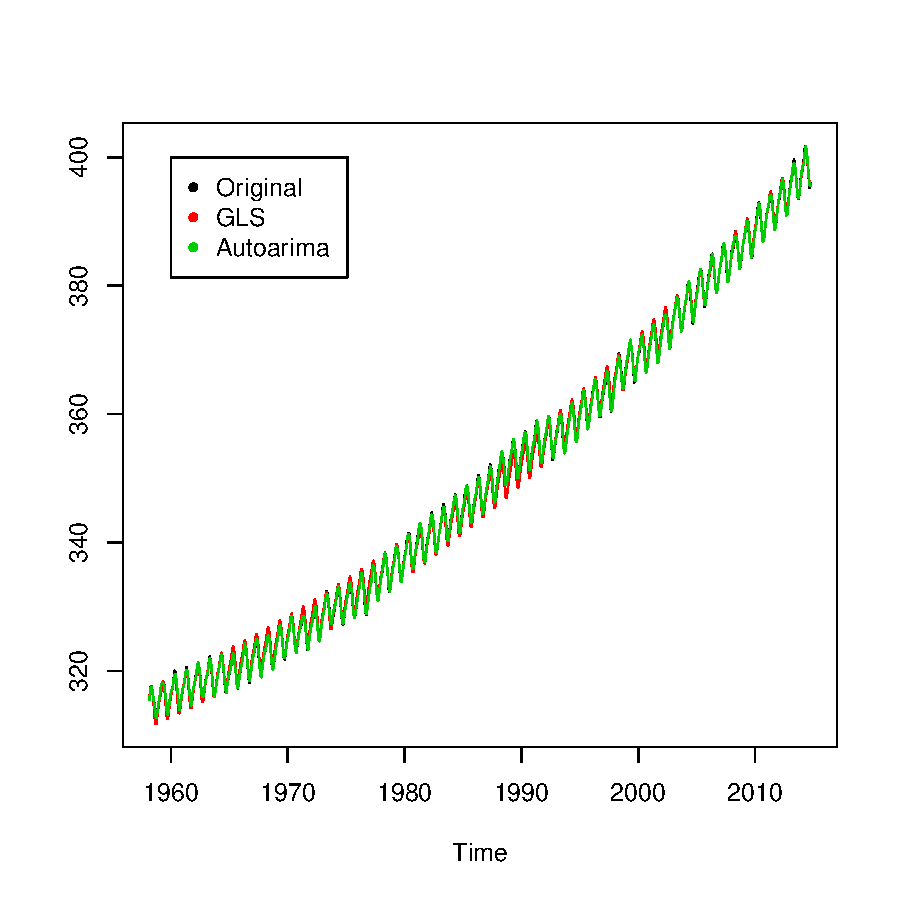
\includegraphics{alleselena-fittedarima}
\caption{Fitted ARIMA values on time series}
\label{fittedarima}
\end{figure}



\begin{figure}[H]
\centering
\begin{Schunk}
\begin{Sinput}
> par(mfrow=c(3,1))
> acf(autoarima$residuals)
> pacf(autoarima$residuals)
> spectrum(autoarima$residuals)
\end{Sinput}
\end{Schunk}
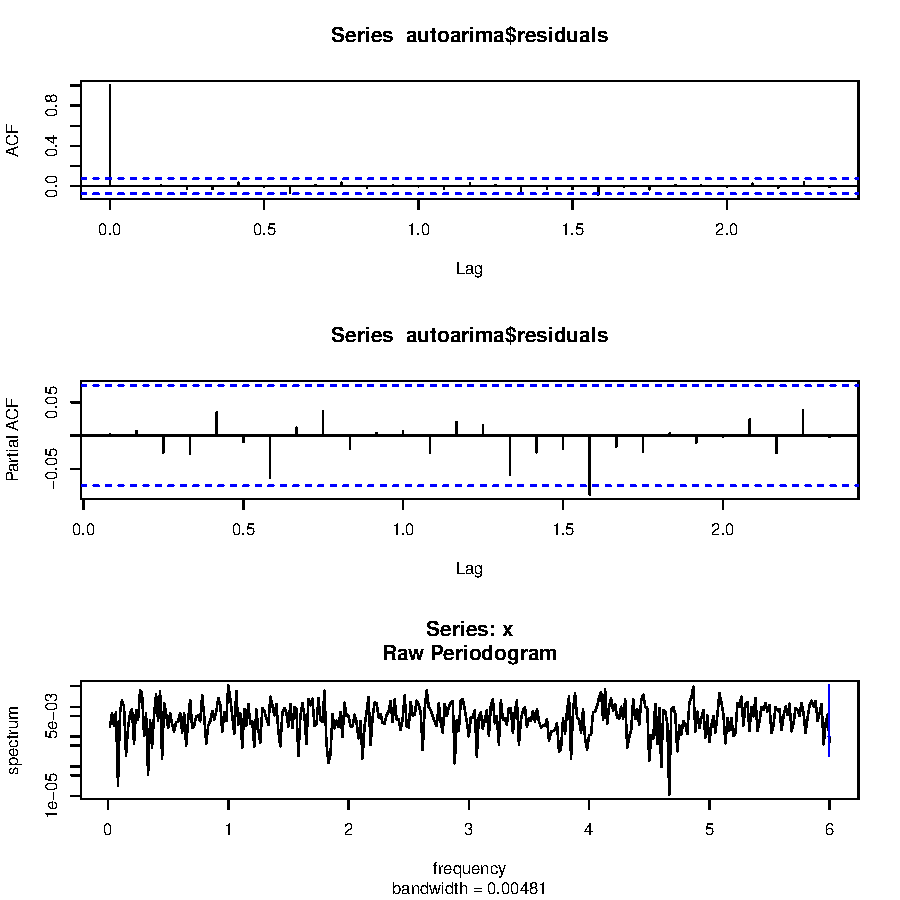
\includegraphics{alleselena-corarima}
\caption{Correlogram for ARIMA}
\label{corarima}
\end{figure}

\begin{figure}[H]
\centering
\begin{Schunk}
\begin{Sinput}
> qqnorm(autoarima$residuals)
> qqline(autoarima$residuals)
\end{Sinput}
\end{Schunk}
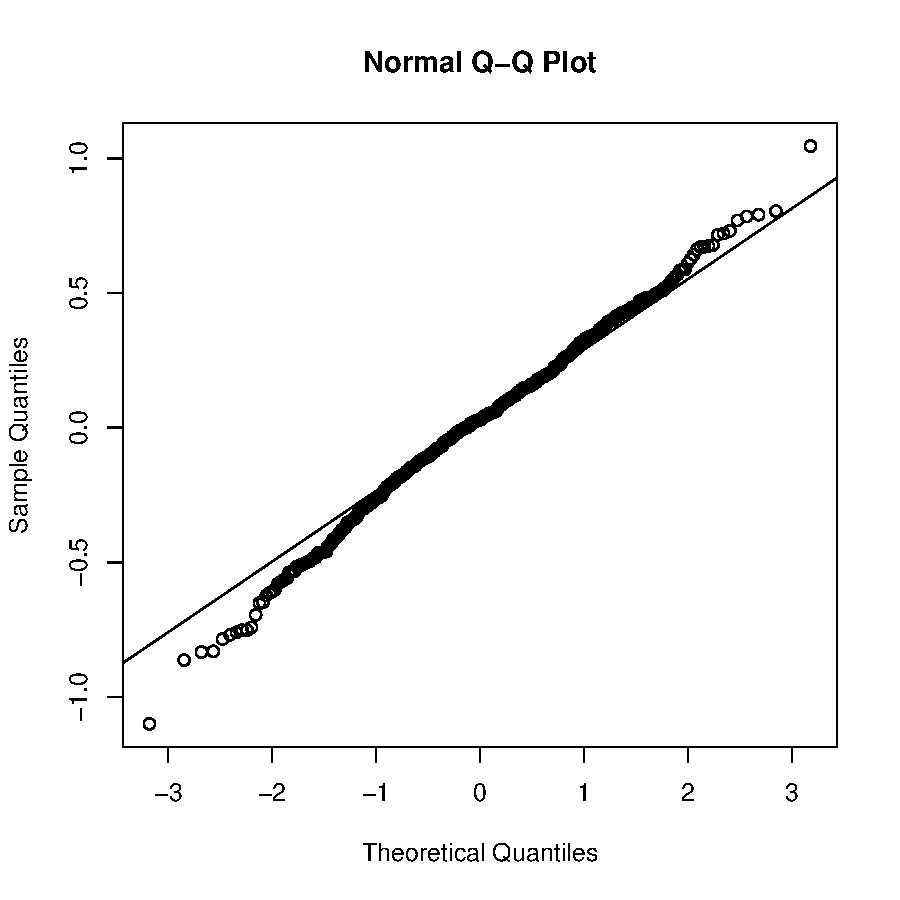
\includegraphics{alleselena-qqarima}
\caption{Correlogram for ARIMA}
\label{qqarima}
\end{figure}

#bestmodel with smallest AIC: 
\begin{Schunk}
\begin{Sinput}
> anova.all = anova( harmonizedgls,harmonizedARMAgls)
> bestmodel= anova.all$call[anova.all$AIC ==min(anova.all$AIC)]
> 
\end{Sinput}
\end{Schunk}

\subsection{Modelling time series with gam}

The GAM generalized additive model could maybe also help finding a quick solution for time series modelling. 

\begin{Schunk}
\begin{Sinput}
> model = gam ( yourts ~ s(time))
> summary(model)
\end{Sinput}
Family: gaussian 
Link function: identity 

Formula:
yourts ~ s(time)

Parametric coefficients:
             Estimate Std. Error t value Pr(>|t|)    
(Intercept) 350.09641    0.08181    4279   <2e-16 ***
---
Signif. codes:  
0 '***' 0.001 '**' 0.01 '*' 0.05 '.' 0.1 ' ' 1

Approximate significance of smooth terms:
          edf Ref.df     F p-value    
s(time) 6.969  8.047 11258  <2e-16 ***
---
Signif. codes:  
0 '***' 0.001 '**' 0.01 '*' 0.05 '.' 0.1 ' ' 1

R-sq.(adj) =  0.993   Deviance explained = 99.3%
GCV = 4.6049  Scale est. = 4.551     n = 680\end{Schunk}

\begin{Schunk}
\begin{Sinput}
> par(mfrow=c(1,1))
> plot.gam(model, residuals=T, scheme=c(2,1), all.terms=T)
\end{Sinput}
\end{Schunk}
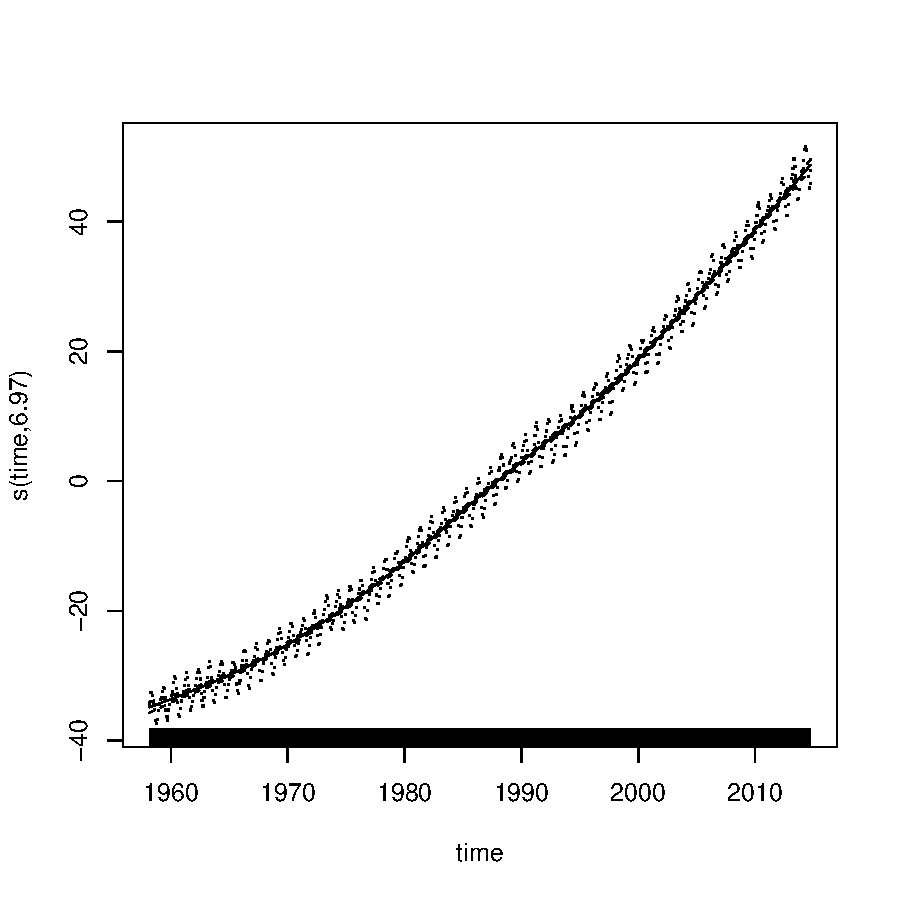
\includegraphics{alleselena-056}

\begin{Schunk}
\begin{Sinput}
> smoothed4gam <- gam(as.numeric(yourts) ~ s(time)  +
                         COS[,1]+SIN[,1]+COS[,2]+SIN[,2]+
                         COS[,3]+SIN[,3]+COS[,4]+SIN[,4]+
                         COS[,5]+SIN[,5]+COS[,6]+SIN[,6]
                       , cor=corARMA(p=2, q=2))
> #summary(smoothed4gam)
> AIC(smoothed4gam)
\end{Sinput}
[1] 926.9626\end{Schunk}

\begin{Schunk}
\begin{Sinput}
> plot(smoothed4gam)
> #8.91 is the edf:array of estimated degrees of freedom for the model terms, calculated for the smoothing term s(time)
\end{Sinput}
\end{Schunk}
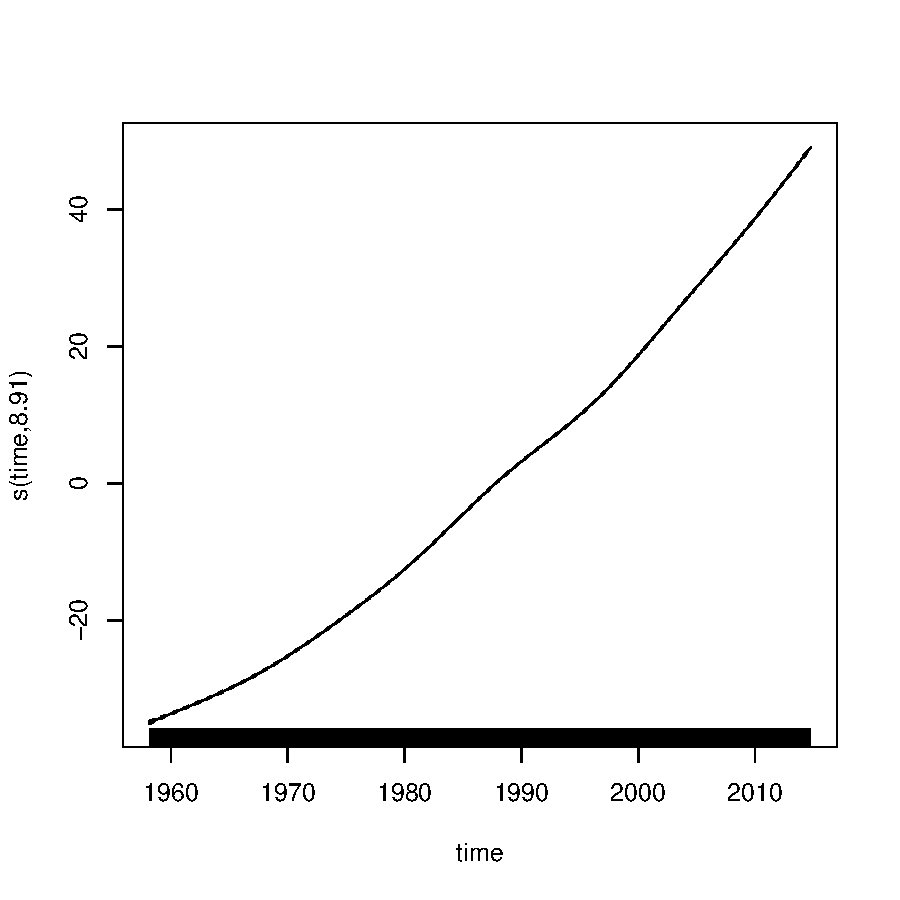
\includegraphics{alleselena-058}



\section{Forecasts}%----------------------------------------------------------------------------------------------------
We have three different options to make ( up to now)
\begin{enumerate}
\item predict()
\item Holt Winters
\item Arima forecasts
\end{enumerate}

If we have a time series that can be described using an additive model,we can short-time forecast using exponential smoothing.\\
Preconditions: forecast errors are uncorrelated and are normally distributed with mean zero and constant variance. To check the forecast errors we have the visualization of the function from above. 

\subsection{Forecast with predict()}
We use our best gls model for this. 
\begin{Schunk}
\begin{Sinput}
> newtime= ts(start=c(2014, 10),end=c(2024,12),deltat=1/12)
> pred = predict(harmonizedARMAgls, newdata=newtime, se=T) 
> TIME <- as.numeric(time)
> time.df <- data.frame(TIME=TIME, COS, SIN)
> colnames(time.df)[-1] <- paste0("V", 1:12)
> smoothed <- gls(as.numeric(yourts) ~ TIME + I(TIME^2) + V1 + V2 + V3 + V4 + V5 
                 +V6 +V7+V8 +V9 +V10 +V11 +V12, 
                 corr=corAR1(acf(dataseasongls$residuals)$acf[2]),
                 data=time.df)
> new.df <- cbind.data.frame(TIME=as.numeric(time(newtime)), 
                            COS=COS[1:123,], SIN=SIN[1:123,])
> colnames(new.df)[-1] <- paste0("V", 1:12)
> pred = predictSE(smoothed, newdata=new.df, se.fit=T)
\end{Sinput}
\end{Schunk}

\begin{Schunk}
\begin{Sinput}
> plot(yourts, type="n",las=1, xlim=c(1960, 2025), 
      ylim=c(300, 450), xlab="Year", ylab="CO2 conc. (ppm)", 
      main="CO2 concentration in the atmosphere")
> grid (NULL,NULL, lty = 6, col = "cornsilk2") 
> points(yourts ,type="l" )
> par(mfrow=c(1,1))
> lines(as.numeric(time(newtime)), pred$fit, col="red")
> F=(pred$fit)
> FSUP=(pred$fit+1.96*pred$se.fit) # make upper conf. int. 
> FSLOW=(pred$fit-1.96*pred$se.fit) # make lower conf. int. 
> lines(new.df$TIME, FSUP,lty=1, col="grey", lwd=3)
> lines(new.df$TIME, FSLOW,lty=1, col="grey", lwd=3)
> lines(new.df$TIME, F, lty=1, col="red", lwd=1)
> legend("topleft",c("forecast for 10 years", "monthly mean data", "CI"), 
        pch=c(20,20), col=c("red", "black", "grey"))
\end{Sinput}
\end{Schunk}
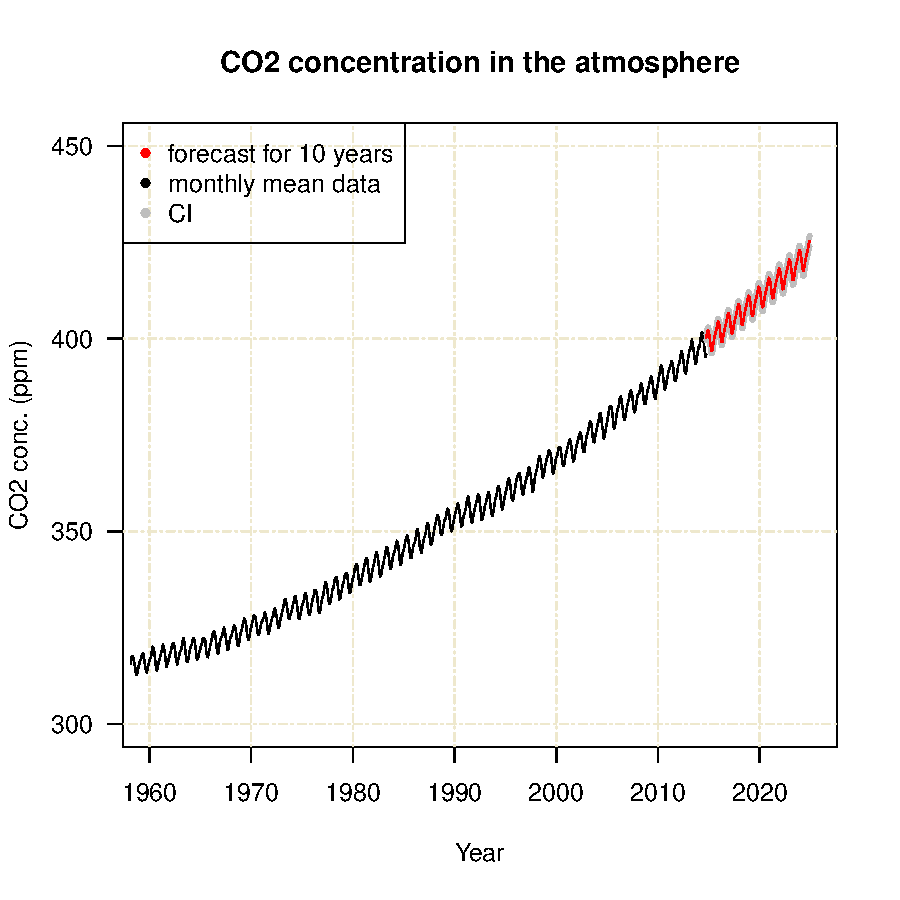
\includegraphics{alleselena-060}


\subsection{Holtwinters forecast function}
Forecasting: from past values (x1,x2,x3,...,xn) want to predict future values x(n+k), \\
holtwinters explanation: \\
#the alpha value tells us the weight of the previous values for the forecasting \\
#values of alpha that are close to 0 mean that little weight is placed on the most recent \\ observations when making forecasts of future values\\
#gamma is for the seasonality \\
if alpha is near 1, little smoothing, at is approx. xt \\
alpha is zero, highly smoothed estimates\\
a = 0.2 compromise figure, change in mean between t-1 and t likel smaller than variance\\

not specify aphla, beta, gamma to include errors, trend and seasonal component in the forecast\\
We use the original data for hw()\\
And predict in the period = 120* 1 month = 10 years\\
\begin{Schunk}
\begin{Sinput}
> forecast <- HoltWinters(yourts)
> forecast10 <- forecast.HoltWinters(forecast,h=120)
\end{Sinput}
\end{Schunk}

Lets see the plot\\
\begin{Schunk}
\begin{Sinput}
> par(mfrow=c(1,1))
> plot.forecast(forecast10,shadecols = "oldstyle")
\end{Sinput}
\end{Schunk}
check for the autocorrelation of the future values\\
\begin{Schunk}
\begin{Sinput}
> par(mfrow=c(2,1))
> acf(forecast10$residuals)
> pacf(forecast10$residuals)
\end{Sinput}
\end{Schunk}
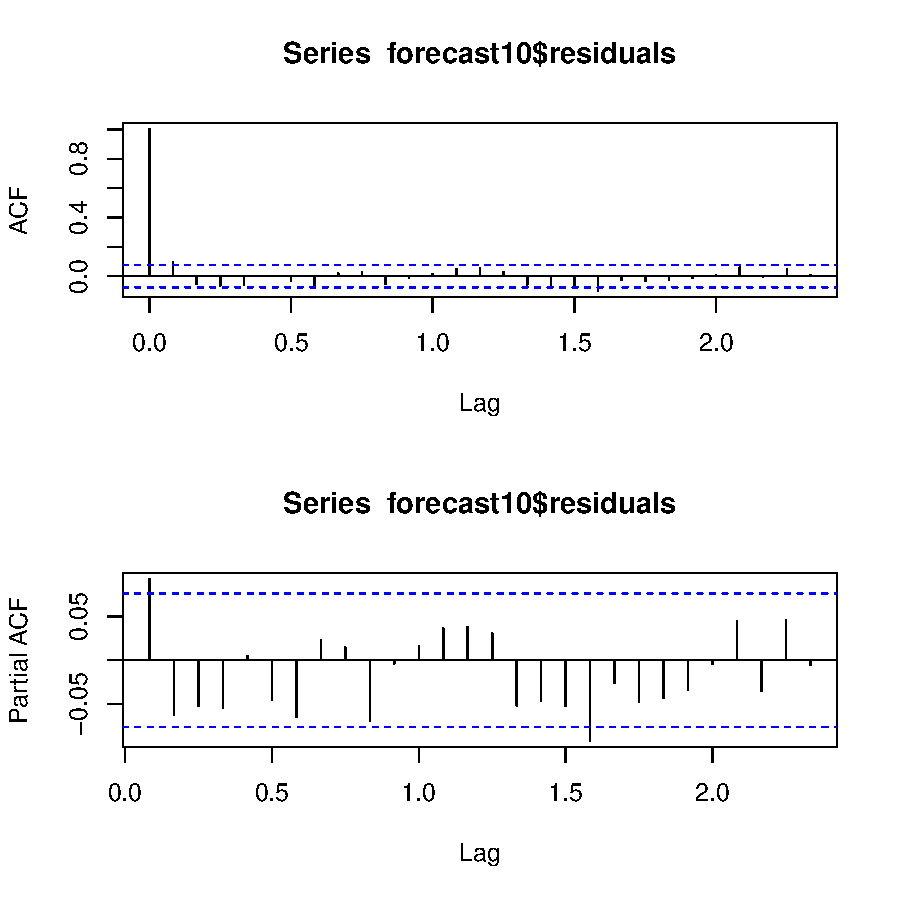
\includegraphics{alleselena-063}
and do the diagnostics on it\\
\begin{Schunk}
\begin{Sinput}
> list = as.list(diagnostics(forecast10))
> print(list)
\end{Sinput}
$`norm. distrb. of residuals`

	Shapiro-Wilk normality test

data:  x$residuals
W = 0.9973, p-value = 0.3574


$`stationarity of residuals`

	Augmented Dickey-Fuller Test

data:  x$residuals
Dickey-Fuller = -9.2646, Lag order = 8, p-value =
0.01
alternative hypothesis: stationary


$`stationarity of fitted values`

	Augmented Dickey-Fuller Test

data:  x$fitted
Dickey-Fuller = -0.8347, Lag order = 8, p-value =
0.9585
alternative hypothesis: stationary


$`autocorrelation of residuals`
[1] 1.80314

$`independence of residuals`

	Box-Ljung test

data:  x$residuals
X-squared = 5.6546, df = 1, p-value = 0.01741\end{Schunk}

\subsection{ARIMA forecast function}
Now we try to forecast with the autoarima function as our bestmodel, which would save alot of time. 

\begin{Schunk}
\begin{Sinput}
> forecast.arima = forecast.Arima(autoarima, h=120) 
\end{Sinput}
\end{Schunk}

\subsection{Comparison of HW and ARIMA}
Lets compare what it better. 

\begin{Schunk}
\begin{Sinput}
> par(mfrow=c(2,1))
> plot.forecast(forecast.arima)
> plot.forecast(forecast10)
\end{Sinput}
\end{Schunk}
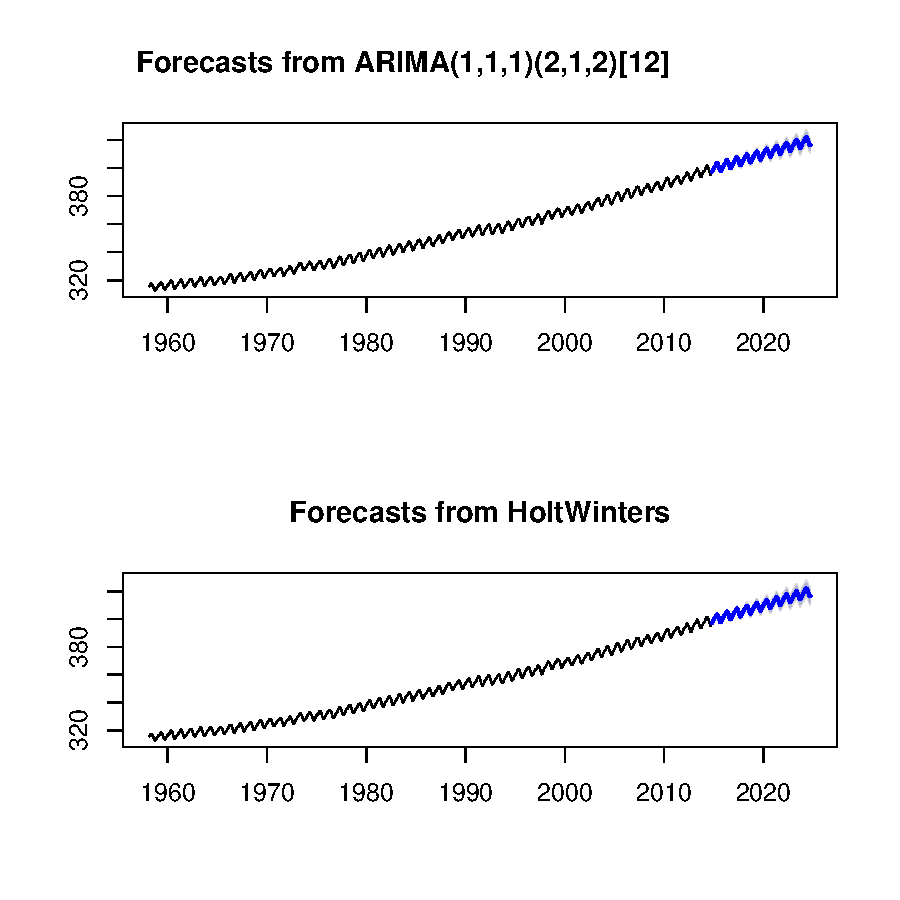
\includegraphics{alleselena-066}

#check for error distirbution with the plotForecastErrors function from above 
\begin{Schunk}
\begin{Sinput}
> par(mfrow=c(1,2))
> plotForecastErrors(forecast10$residuals)
> plotForecastErrors(forecast.arima$residuals)
\end{Sinput}
\end{Schunk}
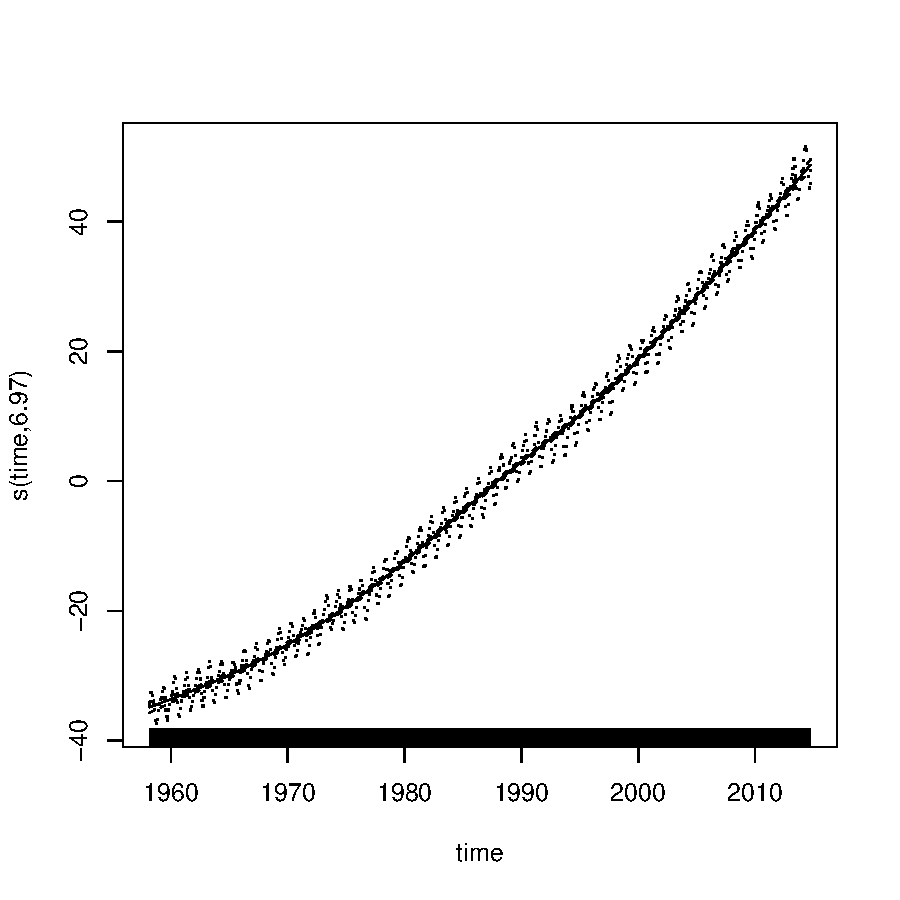
\includegraphics{alleselena-067}
\noindent The histogram of the time series shows that the forecast errors are roughly normally distributed and the mean seems to be close to zero.\\

run diagnostics
\begin{Schunk}
\begin{Sinput}
> list1= as.list(diagnostics(forecast10))
> (list1)
\end{Sinput}
\begin{Soutput}
$`norm. distrb. of residuals`

	Shapiro-Wilk normality test

data:  x$residuals
W = 0.9973, p-value = 0.3574


$`stationarity of residuals`

	Augmented Dickey-Fuller Test

data:  x$residuals
Dickey-Fuller = -9.2646, Lag order = 8, p-value =
0.01
alternative hypothesis: stationary


$`stationarity of fitted values`

	Augmented Dickey-Fuller Test

data:  x$fitted
Dickey-Fuller = -0.8347, Lag order = 8, p-value =
0.9585
alternative hypothesis: stationary


$`autocorrelation of residuals`
[1] 1.80314

$`independence of residuals`

	Box-Ljung test

data:  x$residuals
X-squared = 5.6546, df = 1, p-value = 0.01741
\end{Soutput}
\begin{Sinput}
> list2= as.list(diagnostics(forecast.arima))
> (list2)
\end{Sinput}
\begin{Soutput}
$`norm. distrb. of residuals`

	Shapiro-Wilk normality test

data:  x$residuals
W = 0.9953, p-value = 0.03785


$`stationarity of residuals`

	Augmented Dickey-Fuller Test

data:  x$residuals
Dickey-Fuller = -8.6819, Lag order = 8, p-value =
0.01
alternative hypothesis: stationary


$`stationarity of fitted values`

	Augmented Dickey-Fuller Test

data:  x$fitted
Dickey-Fuller = -0.9422, Lag order = 8, p-value =
0.948
alternative hypothesis: stationary


$`autocorrelation of residuals`
[1] 1.979557

$`independence of residuals`

	Box-Ljung test

data:  x$residuals
X-squared = 0.0046, df = 1, p-value = 0.9461
\end{Soutput}
\end{Schunk}
\linebreak
look at both zoomed in forecasts:
\begin{Schunk}
\begin{Sinput}
> par(mfrow=c(1,2))
> plot(forecast.arima, xlim=c(2010,2025), ylim=c(385,430),shadecols = "oldstyle")
> plot.forecast(forecast10 ,xlim=c(2010,2025), ylim=c(385,430),shadecols = "oldstyle")
\end{Sinput}
\end{Schunk}
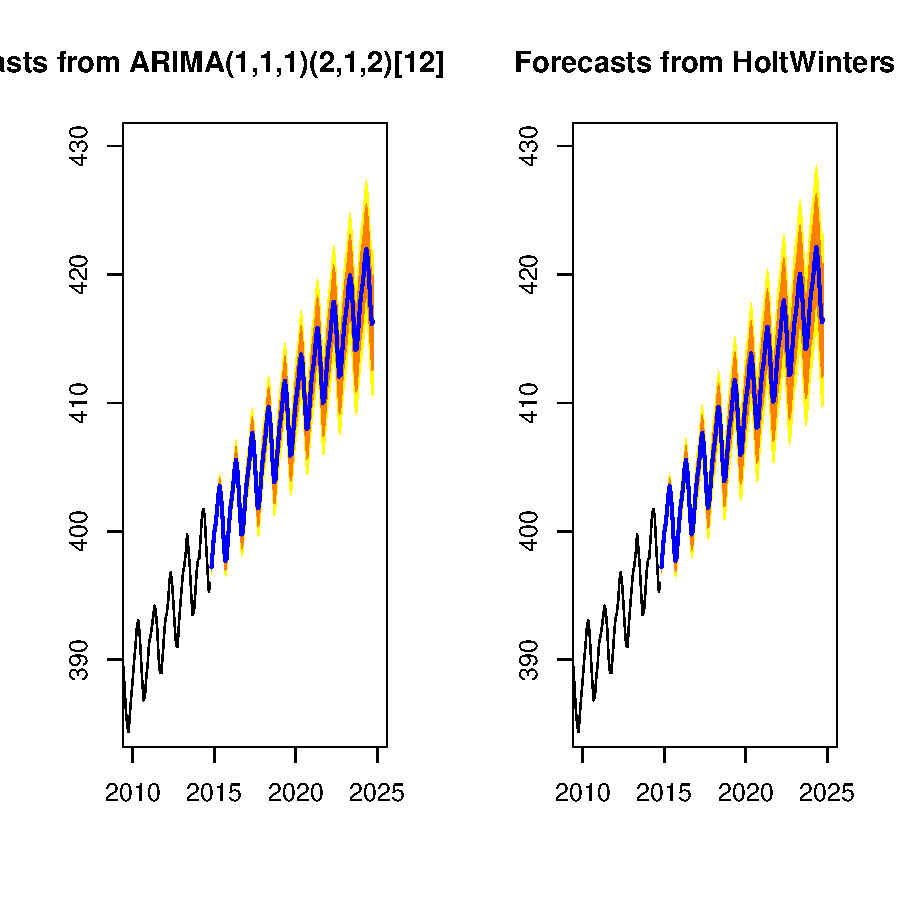
\includegraphics{alleselena-069}



\subsection{Seasonal Decomposition of Time Series by Loess}

Forecasting using stl objects:
\begin{figure}[H]
\centering
\begin{Schunk}
\begin{Sinput}
> plot(stlf(yourts, lambda=0, h =120))
> (tslm(yourts~time(yourts)))
\end{Sinput}
\begin{Soutput}
Call:
lm(formula = formula, data = "yourts", na.action = na.exclude)

Coefficients:
 (Intercept)  time(yourts)  
   -2618.494         1.494  
\end{Soutput}
\end{Schunk}
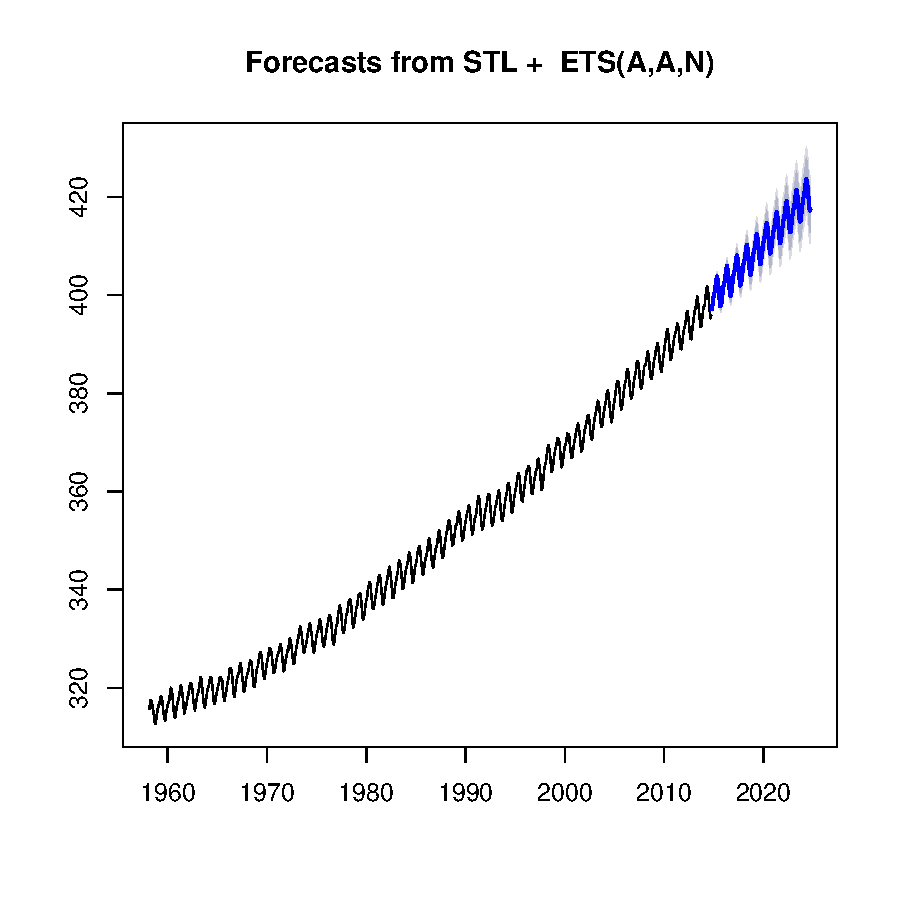
\includegraphics{alleselena-070}
\caption{Forecasting using Loess}
\end{figure}




\section{compabitily with Linux and Windows when working together on a sweave document.}
If you have Linux and have problems working on a same sweave document with Windows users because the line breaks and other text configurations are different, try to type:


\section{Links and Further Reading}%-----------------------------------------------------------------------------------------------
and in:\\
http://cran.r-project.org/web/views/TimeSeries.html\\
Another Exemple Datasets are avaliable at:\\
http://www.comp-engine.org/timeseries/browse-data-by-category\\
https://datamarket.com/data/list/?q=provider:tsdl\\
\section{Acknowledgements}%------------------------------------------------------------------------------------------------------
Don't forget to thank TeX and R and other opensource communities if you use their products! The correct way to cite R is shown when typing ``\texttt{citation()}'', and ``\texttt{citation("mgcv")}'' for packages.

\clearpage
\end{document}
